% **************************************************
% Document Class Definition
% **************************************************
\documentclass[%
    paper=A4,               % paper size --> A4 is default in Germany
    twoside=true,           % onesite or twoside printing
    openright,              % doublepage cleaning ends up right side
    parskip=full,           % spacing value / method for paragraphs
    chapterprefix=true,     % prefix for chapter marks
    11pt,                   % font size
    headings=normal,        % size of headings
    bibliography=totoc,     % include bib in toc
    listof=totoc,           % include listof entries in toc
    titlepage=on,           % own page for each title page
    captions=tableabove,    % display table captions above the float env
    draft=false,            % value for draft version
]{scrreprt}%

% !TEX root = main.tex
% chktex-file 46

% **************************************************
% Files' Character Encoding
% **************************************************
\PassOptionsToPackage{utf8}{inputenc}
\usepackage{inputenc}
\usepackage[ngerman,english]{babel}

% **************************************************
% Information and Commands for Reuse
% **************************************************
\newcommand{\thesisTitle}{Learning to Aggregate on Structured Data}
\newcommand{\thesisName}{Clemens Damke}
\newcommand{\thesisMatNr}{7011488}
\newcommand{\thesisSubject}{Master Thesis}
\newcommand{\thesisDate}{\today}
\newcommand{\thesisVersion}{Draft}

\newcommand{\thesisFirstReviewer}{Prof.~Dr.~Eyke Hüllermeier}
\newcommand{\thesisFirstReviewerUniversity}{Paderborn University}
\newcommand{\thesisFirstReviewerDepartment}{Intelligent Systems and Machine Learning Group (ISG)}

\newcommand{\thesisSecondReviewer}{Prof.~Dr.~Axel-Cyrille Ngonga Ngomo}
\newcommand{\thesisSecondReviewerUniversity}{Paderborn University}
\newcommand{\thesisSecondReviewerDepartment}{Data Science Group (DICE)}

\newcommand{\thesisSupervisor}{Vitalik Melnikov}

\newcommand{\thesisUniversity}{Paderborn University}
\newcommand{\thesisUniversityDepartment}{Department of Electrical Engineering, Computer Science and Mathematics}
\newcommand{\thesisUniversityInstitute}{Heinz Nixdorf Institute}
\newcommand{\thesisUniversityGroup}{Intelligent Systems and Machine Learning Group (ISG)}
\newcommand{\thesisUniversityStreetAddress}{Warburger Straße 100}
\newcommand{\thesisUniversityPostalCode}{33098}
\newcommand{\thesisUniversityCity}{Paderborn}


% **************************************************
% Debug LaTeX Information
% **************************************************
%\listfiles


% **************************************************
% Load and Configure Packages
% **************************************************

% Colors:
\usepackage[usenames, dvipsnames, svgnames, table]{xcolor}

\definecolor{t_blue}{HTML}{355fb3}
\definecolor{t_red}{HTML}{b33535}
\definecolor{t_green}{HTML}{3bb335}
\definecolor{t_yellow}{HTML}{b39735}
\definecolor{t_darkblue}{HTML}{1e3666}
\definecolor{t_darkgreen}{HTML}{22661e}
\definecolor{t_darkyellow}{HTML}{66571e}
\definecolor{t_lightblue}{HTML}{8ea7d7}

% Code snippets:
\usepackage{minted}
\usepackage{etoolbox,xpatch}
\makeatletter
\AtBeginEnvironment{minted}{\dontdofcolorbox}
\def\dontdofcolorbox{\renewcommand\fcolorbox[4][]{##4}}
\xpatchcmd{\inputminted}{\minted@fvset}{\minted@fvset\dontdofcolorbox}{}{}
\makeatother
\setminted{
	fontsize=\footnotesize,
	numbers=left,
	tabsize=4,
	breaklines=true
}

\PassOptionsToPackage{% setup clean thesis style
    figuresep=space,
    sansserif=false,
    hangfigurecaption=false,
    hangsection=true,
    hangsubsection=true,
    colorize=full,
    colortheme=custom,
	colormain=t_darkblue,
	coloraccessory=t_blue,
    bibsys=bibtex,
    bibfile=literature,
    bibstyle=alphabetic,
    wrapfooter=false,
}{cleanthesis}
\usepackage{cleanthesis}

\usepackage{mathtools}
\usepackage{amssymb}
\usepackage{amsthm}
\usepackage{thmtools}
\usepackage{bm}
\usepackage{bbm}
\usepackage{dsfont}
\usepackage{centernot}
\usepackage{breqn}
\usepackage{nicefrac}
\usepackage{wasysym}
\newcommand\numberthis{\addtocounter{equation}{1}\tag{\theequation}}
\newcommand*{\dblbrace}[2][]{#1{#2}\ifthenelse{\equal{#1}{}}{\mskip-6mu}{\mskip-8mu}#1{#2}}
\newcommand*{\ldblbrace}[1][]{\dblbrace[#1]{\{}}
\newcommand*{\rdblbrace}[1][]{\dblbrace[#1]{\}}}
\newcommand*\dif{\mathop{}\!\mathrm{d}}

\makeatletter
\renewenvironment{proof}[1][\proofname]{\par
	\pushQED{\qed}%
	\topsep-10pt
	\trivlist%
	\item[\hskip\labelsep% chktex 41
		\itshape%
		#1\@addpunct{.}%
	]\ignorespaces%
}{%
  \popQED\endtrivlist\@endpefalse% chktex 21
}
\def\th@plain{\thm@preskip\parskip\thm@postskip0pt\itshape} % chktex 6
\def\th@definition{\thm@preskip\parskip\thm@postskip0pt\normalfont}
\def\th@remark{\thm@headfont{\itshape}\normalfont\thm@preskip\parskip\thm@postskip0pt} % chktex 6
\makeatother

\usepackage{pifont}
\usepackage{graphicx}
\usepackage{tikz}
\usetikzlibrary{arrows,positioning}
\usetikzlibrary{calc}

\usepackage{pgfplots}
\usepackage{pgfplotstable}
\pgfplotsset{compat=1.14}
\usepgfplotslibrary{dateplot, statistics}
\pgfplotsset{
    cycle list={t_blue\\t_red\\t_green\\},
}

\usepackage{listings}
\lstset{basicstyle=\ttfamily,breaklines=true}

\usepackage{tasks}
\settasks{counter-format=tsk[1].}

\usepackage{acro}
\acsetup{first-long-format=\slshape} % chktex 6
\acsetup{single}
\acsetup{use-barriers}
\acsetup{reset-at-barriers}

\usepackage{stmaryrd}
\usepackage{multicol}
\usepackage{pbox}
\usepackage{longtable}
\usepackage{booktabs}
\usepackage{csvsimple}
\usepackage{siunitx}
\usepackage[nameinlink]{cleveref}

\hypersetup{% setup the hyperref-package options
    pdftitle={\thesisTitle},    %   - title (PDF meta)
    pdfsubject={\thesisSubject},%   - subject (PDF meta)
    pdfauthor={\thesisName},    %   - author (PDF meta)
    plainpages=false,           %   -
    colorlinks=false,           %   - colorize links?
    pdfborder={0 0 0},          %   -
    breaklinks=true,            %   - allow line break inside links
    bookmarksnumbered=true,     %
    bookmarksopen=true,         %
	hypertexnames=true,         %
}

% Custom commands:
\newcommand{\tikzmark}[1]{\tikz[overlay,remember picture] \node (#1) {};} % chktex 1
\newcommand{\dac}[3]{\DeclareAcronym{#1}{short = #2, long = #3}}
\newcommand*\circled[2][1pt]{\tikz[baseline=(char.base)]{ % chktex 36
    \node[shape=circle,draw,inner sep=#1] (char) {#2};}}
\newcommand*{\badgeboxinline}[2][black]{\fcolorbox{#1}{white}{\textsf{%
	\small\,% chktex 21
	\ifthenelse{\equal{\detokenize{#1}}{\detokenize{t_yellow}}}{\textcolor{t_darkyellow}{#2}}{\textcolor{#1}{#2}}\,}}} % chktex 21
\newcommand*{\badgebox}[2][black]{\hspace*{\fill}\badgeboxinline[#1]{#2}}
\newcommand{\cmark}{\ding{51}}
\newcommand{\xmark}{\ding{55}}
\providecommand\rightarrowRHD{\mathrel{\relbar\mathrel{\mkern-8mu\RHD}}}

\newcommand{\sourceinline}[2][source]{{\scriptsize\textsc{#1:~\cite{#2}}}}
\newcommand{\source}[2][source]{\hspace*{\fill}\sourceinline[#1]{#2}}
\newcommand{\cfullref}[2][, ]{\cref{#2}#1\cpageref{#2}}

\newcounter{daggerfootnote}
\newcommand*{\daggerfootnote}[1]{%
\setcounter{daggerfootnote}{\value{footnote}}%
\renewcommand*{\thefootnote}{\fnsymbol{footnote}}%
\footnote[2]{#1}%
\setcounter{footnote}{\value{daggerfootnote}}%
\renewcommand*{\thefootnote}{\arabic{footnote}}}

\DeclareMathOperator{\Tr}{Tr}
\DeclareMathOperator{\mean}{mean}
\DeclareMathOperator{\wmean}{wmean}
\DeclareMathOperator{\wmaj}{wmaj}
\DeclareMathOperator{\sgn}{sgn}
\DeclareMathOperator{\set}{set}

\theoremstyle{plain}
\newtheorem{thm}{Theorem}[chapter]
\newtheorem{prop}[thm]{Proposition}
\newtheorem{lem}[thm]{Lemma}
\newtheorem{fact}[thm]{Fact}
\newtheorem{cor}[thm]{Corollary}

\theoremstyle{definition}
\newtheorem{defn}[thm]{Definition}

% !TEX root = ../main.tex

% General:
\dac{ml}{ML}{machine learning}

% Other learners:
\dac{nn}{NN}{neural network}
\dac{lm}{LM}{logistic model}
\dac{svm}{SVM}{support vector machine}
\dac{mlp}{MLP}{multilayer perceptron}
\dac{cnn}{CNN}{convolutional neural network}

% Graph Kernel:
\dac{gk}{GK}{graph kernel}

% Graph NN:
\dac{gnn}{GNN}{graph neural network}
\dac{gcnn}{GCNN}{graph convolutional neural network}

\bibliography{literature}

% **************************************************
% Document CONTENT
% **************************************************
\begin{document}

% --------------------------
% rename document parts
% --------------------------

\newcommand{\fixedinput}{\input}

% --------------------------
% Front matter
% --------------------------
\pagenumbering{roman}			% roman page numbing (invisible for empty page style)
\pagestyle{empty}				% no header or footers
% !TEX root = ../main.tex
%
% ------------------------------------  --> cover title page
\begin{titlepage}
	\pdfbookmark[0]{Cover}{Cover}
	\sffamily\
	\flushright\
	\hfill
	\vfill
	{\color{ctcolortitle}\LARGE\thesisTitle\ \par}
	\rule[5pt]{\textwidth}{.4pt} \par
	{\Large\thesisName}
	\vfill
	\textit{\large\thesisDate}
\end{titlepage}


% ------------------------------------  --> main title page
\begin{titlepage}
	\pdfbookmark[0]{Titlepage}{Titlepage}
	\sffamily\

	\begin{figure}
	\begin{minipage}[t]{8.5cm}
	\includegraphics[height=1.8cm]{gfx/upb_1E}\\
	\textsf{\small{\hspace*{1.3cm}Department of Electrical Engineering,\\
	\hspace*{1.3cm}Computer Science and Mathematics\\
%		\hspace*{1.3cm}Institute of Computer Science\\
		\hspace*{1.3cm}Warburger Straße 100 \\
		\hspace*{1.3cm}33098 Paderborn
		}}
	\end{minipage}
	\hfill
	\begin{minipage}[t]{4.7cm}
	\includegraphics[height=1.8cm]{gfx/is-logo-klein}\\
	\textsf{\small{
		\hspace*{0.1cm}Intelligent Systems and\\
		\hspace*{0.1cm}Machine Learning Group (ISG)
	}}
	\end{minipage}
	\end{figure}

	\centering

	\vfill
	{\large \thesisSubject} \\[5mm]
	{\LARGE \color{ctcolortitle}\textbf{\thesisTitle} \\[10mm]}
	{\Large \thesisName} \\

	\vfill
	\begin{minipage}[t]{.27\textwidth}
		\raggedleft\
		\textit{1. Reviewer}
	\end{minipage}
	\hspace*{15pt}
	\begin{minipage}[t]{.65\textwidth}
		{\Large \thesisFirstReviewer} \\
	  	{\small \thesisFirstReviewerDepartment} \\[-1mm]
		{\small \thesisFirstReviewerUniversity}
	\end{minipage} \\[5mm]
	\begin{minipage}[t]{.27\textwidth}
		\raggedleft\
		\textit{2. Reviewer}
	\end{minipage}
	\hspace*{15pt}
	\begin{minipage}[t]{.65\textwidth}
		{\Large \thesisSecondReviewer} \\
	  	{\small \thesisSecondReviewerDepartment} \\[-1mm]
		{\small \thesisSecondReviewerUniversity}
	\end{minipage} \\[15mm]

	\thesisDate\\ % chktex 21

\end{titlepage}


% ------------------------------------  --> lower title back for single page layout
\hfill
\vfill
{
	\small
	\textbf{\thesisName} \\
	\textit{\thesisTitle} \\
	\thesisSubject, \thesisDate\\ % chktex 21
	Reviewers: \thesisFirstReviewer\ and \thesisSecondReviewer\\ % chktex 21
	Supervisor: \thesisSupervisor\\[1.5em] % chktex 21
	\textbf{\thesisUniversity} \\
	\textit{\thesisUniversityGroup} \\
	\thesisUniversityInstitute\\ % chktex 21
	\thesisUniversityDepartment\\ % chktex 21
	\thesisUniversityStreetAddress\\ % chktex 21
	\thesisUniversityPostalCode\ \thesisUniversityCity\
}
		% INCLUDE: all titlepages
\cleardoublepage\

\pagestyle{plain}				% display just page numbers
%!TEX root = ../main.tex
%
\pdfbookmark[0]{Abstract}{Abstract}
\chapter*{Abstract}%
\label{sec:abstract}
\vspace*{-10mm}

This thesis describes the research field of \acl{gcr} from the perspective of the \ac{lta} problem.
It formally characterizes a selection of state-of-the-art \textit{graph kernels} and \acp{gnn} as instances of \ac{lta}.
Those characterizations are shown to be limited by the way in which they decompose graphs.
To overcome this limitation, an avenue for a more ``\acs{lta}-like'' \ac{gnn} is provided in form of so-called \textit{learned edge filters}.
To realize edge filters, the novel \textit{2-\acs*{wl}-\acs*{gnn}} model is proposed;
it is inspired by the two-dimensional \ac{wl} algorithm and proven to be strictly more expressive than existing \ac{gnn} approaches which are bounded by the more restrictive one-dimensional \ac{wl} algorithm.
		% INCLUDE: the abstracts (english and german)
\acbarrier\cleardoublepage\
%
\setcounter{tocdepth}{2}		% define depth of toc
\tableofcontents				% display table of contents
\cleardoublepage\
% --------------------------
% Body matter
% --------------------------
\pagestyle{maincontentstyle} 	% fancy header and footer

% !TEX root = ../main.tex
% chktex-file 46
\chapter{Introduction}%
\label{sec:intro}

\pagenumbering{arabic}			% arabic page numbering
\setcounter{page}{1}			% set page counter

\section{Motivation}%
\label{sec:intro:motivation}

The field of \ac{ml} on graph-structured data has applications in many domains due to the general expressive power of graphs.
The three most common types of graph~\ac{ml} problems are
\begin{enumerate}[label=\textbf{\arabic*.}]
	\item \textbf{Link prediction:}
		A graph with an incomplete edge set is given and the missing edges have to be predicted.
		The suggestion of potential friends in a social network is a typical example for this.
	\item \textbf{Vertex classification \& regression:}
		Here a class or a score has to be predicted for each vertex of a graph.
		In social graphs this corresponds to the prediction of properties of individuals, e.g.\ personal preferences or gender.
		Another example is the prediction of the amount of traffic at the intersections of a street network.
	\item \textbf{Graph classification \& regression:}
		In this final problem type a single global class or continuous value has to be predicted for an input graph.
		The canonical example for this is the prediction of properties of molecule graphs, e.g.\ the toxicity or solubility of a chemical.
\end{enumerate}
In this thesis we will focus on the last problem type, \ac{gcr}.
An \ac{ml} method for this problem has to accept graphs of varying size and should be permutation invariant wrt.\ the order in which graph vertices are provided.
Those requirements are not met by the commonly used learners that only accept fixed-size feature vectors as their input, e.g.\ \acp{lm}, \acp{svm} or \acp{mlp}.

A \ac{gcr} method has to account for two central aspects of the problem:
\begin{enumerate*}
	\item Local structural analysis and
	\item global aggregation
\end{enumerate*}.
The first aspect is about the extraction of relevant features of substructures of the input graph.
The latter is about the way in which the local features are combined into a final class or regression value.
The existing \ac{gcr} methods are mostly motivated by local structural graph analysis.
The aspect of global aggregation on the other hand is less emphasized by those methods.

There is however a separate branch of research that specifically looks at the problem of learning aggregation functions, called \ac{lta}.
Current \ac{lta} approaches explicitly learn an aggregation functions for sets which can be interpreted as graphs without edges.
The motivation for this thesis is to generalize \ac{lta} from sets to arbitrary graphs.
The overall goal is to combine the aggregation learning perspective with existing \ac{gcr} methods.

\section{Goals}%
\label{sec:intro:goals}

To extend \ac{lta} to graphs, three goals have to be achieved:
\begin{enumerate}[label=\textbf{\arabic*.}]
	\item \textbf{Formalization of \ac{lta}:}
		Before \ac{lta} can be extended, its essential characteristics have to be defined.
		Those characteristics should provide the terminology to formally capture the differences and similarities between \ac{lta} and existing \ac{gcr} methods.
	\item \textbf{Give an \ac{lta} interpretation of \ac{gcr} methods:}
		Using the \ac{lta} formalization, representative \ac{gcr} approaches should be restated as \ac{lta} instances.
		Currently there is no comprehensive formulation of the relation between both fields of research;
		this is addressed by the the second goal.
	\item \textbf{Define an \ac{lta} method for graphs:}
		Using the \ac{lta} perspective on \ac{gcr}, hidden assumptions of the existing approaches should become clear and in which way they share the assumptions of \ac{lta}.
		The last goal is to use those insights to formulate an \ac{lta}-\ac{gcr} method that combines ideas from the existing approaches with the \ac{lta} assumptions.
\end{enumerate}

\section{Structure}%
\label{sec:intro:structure}

\paragraph{\Cref{sec:related}: \nameref{sec:related}}

\paragraph{\Cref{sec:ltag}: \nameref{sec:ltag}}

\paragraph{\Cref{sec:eval}: \nameref{sec:eval}}

\paragraph{\Cref{sec:conclusion}: \nameref{sec:conclusion}}

\section{Formal Notation}%
\label{sec:intro:notation}

% !TEX root = ../main.tex
% chktex-file 46
\chapter{Related Work}%
\label{sec:related}

\section{Learning to Aggregate}%
\label{sec:related:lta}

\section{Graph Kernels}%
\label{sec:related:gk}

\section{Graph Neural Networks}%
\label{sec:related:gnn}

\subsection{Spatial GNNs}%
\label{sec:related:gnn:spatial}

\subsection{Spectral GNNs}%
\label{sec:related:gnn:spectral}

%!TEX root = ../main.tex
% chktex-file 46
\chapter{Learning to Aggregate on Graphs}%
\label{sec:ltag}

In the previous chapter an introduction to two separate fields of research was given:
\begin{enumerate*}
	\item \Acf{lta},
	\item \Acf{gcr}
\end{enumerate*}.
In this chapter we will combine them and define an extension of \ac{lta} to the \ac{gcr} problem.
This will be done in three steps:
\begin{enumerate}
	\item We begin with a formal definition of what actually constitutes an \ac{lta} method as opposed to non-\acs{lta} methods.
	\item Using this definition, we will see that some of the previously described \ac{gcr} methods can be interpreted as \ac{lta} variants under certain conditions.
	\item Finally a novel \acs{lta}-inspired \ac{gcnn} architecture will be described.
\end{enumerate}

\section{A Generalized Definition of \acs*{lta}}%
\label{sec:ltag:definition}

In order to formally define \ac{lta}, we must first decide on its defining characteristic.
We propose that this characteristic should be the \textit{localized explainability} of \ac{lta} predictions.
As seen in \cref{sec:related:lta}, an \ac{lta} score $y_{C} \in \mathcal{Y}$ for some multiset composition $C = \ldblbrace c_1, \dots, c_n \rdblbrace$ can always be tracked back to a set of local constituent scores $y_1, \dots, y_n \in \mathcal{Y}$.
Under the assumption that each constituent $c_i$ represents some human interpretable object, a composition's score $y_{C}$ can therefore be explained by the presence of certain indicative constituents/objects $c_i$.

Based on this intuition we now give a generalized definition of \ac{lta} which applies to unstructured as well as structured input data.
We assume that all compositions are represented by graphs $G \in \mathcal{G}$;
an unstructured input is represented by a graph with one vertex per constituent ($\mathcal{V}_G = \{ v_{c_1}, \dots, v_{c_n} \}$) and no edges ($\mathcal{E}_G = \emptyset$).
Each composition has some target score $y_G \in \mathcal{Y}$ which could be a discrete class or continuous value.
An \textit{\ac{lta} model} $h: \mathcal{G} \to \mathcal{Y}$ assigns predictions $\hat{y}_G \in \mathcal{Y}$ to compositions $G$ which ideally correspond to the true score $y_G$.
Such a model must satisfy three criteria:
\begin{enumerate}[label=\textbf{\arabic*.}]
	\item \textbf{Decomposition:}
		A given composition $G$ must be decomposed into a set of constituents $c_{G,i}$ via a \textit{decomposition function} $\psi: \mathcal{G} \to \mathcal{P}(\mathcal{G})$.
		\begin{defn}\label{defn:ltag:decomp}
			$\psi$ is a \textit{decomposition function} iff.\ it splits a graph into a subset of its subgraphs, i.e.\ $\forall G \in \mathcal{G}: \forall c_{G,i} \in \psi(G): \exists s \in \mathcal{P}(\mathcal{V}_G): c_{G,i} = G[s]$.
		\end{defn}
		Note that the strict equality $c_{G,i} = G[s]$ is used in \cref{defn:ltag:decomp} instead of just requiring subgraph isomorphism ($c_{G,i} \simeq G[s]$) because a constituent $c_{G,i}$ represents a specific localized subgraph of a structured composition.

		In the existing unstructured \ac{lta} approaches the decomposition function is implicitly defined as $\psi(G) \coloneqq {\{ G[v_{c_i}] \}}_{v_{c_i} \in \mathcal{V}_G}$ since each vertex $v_{c_i}$ corresponds to an interpretable constituent $c_i$ by definition.
		For structured data however, a split into individual vertices is typically not appropriate.
		Molecular graphs from chemical datasets for example are meaningfully characterized by the presence of so-called \textit{functional groups} consisting of multiple bonded atoms while a characterization on the level of individual atoms is generally less meaningful~\cite{McNaught1997}.
	\item \textbf{Local evaluation:}
		The constituents $c_{G, i} \in \psi(G)$ must be evaluated via some function $f: \mathcal{G} \to \mathcal{Y} \times \mathbb{R}$.
		This \textit{evaluation function} assigns a prediction $\hat{y}_{G, i} \in \mathcal{Y}$ and a weight $w_{G, i} \in \mathbb{R}$ to each constituent.
		A constituent's weight $w_{G, i}$ can intuitively be interpreted as a measure of the confidence that the local prediction $\hat{y}_{G, i}$ is indicative of the composition's global target score $y_G$.
		Learning local predictions and weights for all possible constituents is called the \textit{disaggregation problem}.

		Note that there are no explicit constituent weights in the existing unstructured \ac{lta} approaches (i.e.\ implicitly all $w_{G, i} = 1$) because the explicitly given constituents are assumed to be equally indicative of $y_G$.
		For structured data however, where the decomposition $\psi(G)$ is not given as part of the input, this assumption does not necessarily hold.
		By weighting the constituents, an \ac{lta} model can reduce the relevance or even ignore constituents that turn out to be irrelevant for the compositions target score $y_G$.
	\item \textbf{Aggregation:}
		Lastly a \textit{weighted aggregation function} $\mathcal{A}: {(\mathcal{Y} \times \mathbb{R}_{\geq 0})}^{*} \to \mathcal{Y}$ must be applied.
		It combines the multiset of local constituent predictions and non-negative weights into a single global composition prediction.
		\begin{defn}\label{defn:ltag:weighted-agg}
			We call $\mathcal{A}$ a \textit{weighted aggregation function} iff.\ it satisfies
			\begin{align*}
				\text{idempotency: } & \exists \eta > 0: \forall y \in \mathcal{Y}, w \in \mathbb{R}_{\geq 0}^n\text{ s.t. }{\max w} \geq \eta: \mathcal{A}({\ldblbrace (y, w_i) \rdblbrace}_{i=1}^n) = y \\
				\land\text{ zero invar.: } & \forall y_0 \in \mathcal{Y}, S = {\ldblbrace (y_i, w_i) \rdblbrace}_{i=1}^n: \mathcal{A}(S \cup \{ (y_0, 0) \}) = \mathcal{A}(S) \text{.}
			\end{align*}
		\end{defn}
		{\setlength{\parskip}{0pt}The idempotency constraint requires aggregation functions to agree with uniform input scores $y$ if at least one input is weighted above some threshold $\eta$.
		The zero invariance constraint requires aggregation functions to ignore inputs with zero weight.
		Exemplary weighted aggregation function are:}
		\begin{itemize}
			\item The \textit{weighted mean} function $\wmean({\ldblbrace (y_i, w_i) \rdblbrace}_{i=1}^n) \coloneqq \sum_{i=1}^n w_i y_i$ which requires $\sum w_i = 1$, $w_i \in [0, 1]$ and the existence of some scalar multiplication operator $\cdot: \mathbb{R} \times \mathcal{Y} \to \mathcal{Y}$, typically from some subfield $\mathcal{Y} \subseteq \mathbb{R}$ or possibly also some vector subspace $\mathcal{Y} \subseteq \mathbb{R}^d$.
			\item Another basic weighted aggregator is the \textit{weighted majority vote} function $\wmaj({\ldblbrace (y_i, w_i) \rdblbrace}_{i=1}^n) \coloneqq {\arg\max}_{y \in \mathcal{Y}} \sum_{y_i = y} w_i$ which returns the input with the highest total weight.
				Unlike $\wmean$ it can also be applied to score domains $\mathcal{Y}$ without a multiplication operator, e.g.\ sets of discrete classes.
			\item Alternatively an unweighted aggregation function like $\min$, $\max$, $\mean$ or \ac{owa}\footnote{
				Even though \ac{owa} uses weights, it does not get those weights as part of the input and is therefore considered to be unweighted in this context.
			} also trivially satisfies \cref{defn:ltag:weighted-agg} if all inputs $y_i$ with $w_i = 0$ are filtered out and the weights for all remaining inputs are ignored.
		\end{itemize}
\end{enumerate}
\begin{figure}[ht]
	\centering
	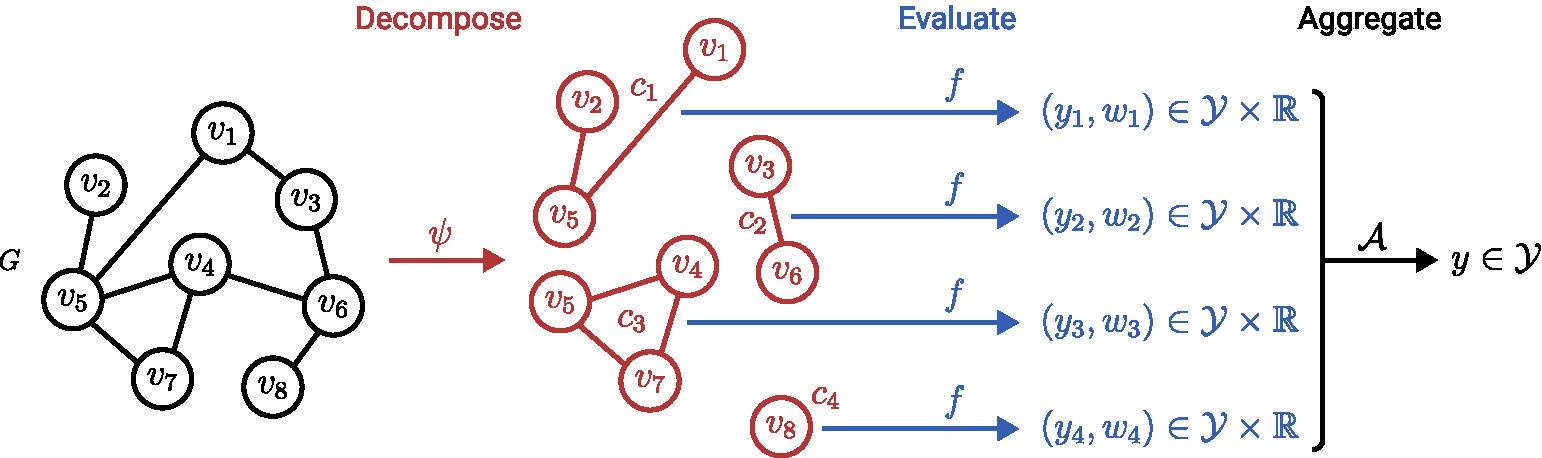
\includegraphics[width=\linewidth]{gfx/graph-lta/ltag-overview.pdf}
	\caption{
		Overview of the generalized \ac{lta} architecture for structured data.
	}\label{fig:ltag:ltag-overview}
\end{figure}
Based on the notion of decomposition, local evaluation and aggregation we can now define the concept of \textit{\ac{lta} formulations}.
\begin{defn}
	A model $h: \mathcal{G} \to \mathcal{Y}$ is in an \textit{\ac{lta} formulation} iff.\ it is expressed as
	\begin{align*}
		h(G) \coloneqq \mathcal{A}(\ldblbrace f(c_{G,i})\, |\, c_{G,i} \in \psi(G) \rdblbrace) \quad\text{with $\psi$, $f$ and $\mathcal{A}$ as defined above.}
	\end{align*}
\end{defn}
Note that every model $h: \mathcal{G} \to \mathcal{Y}$ has a trivial recursive \ac{lta} formulation by choosing $\psi(G) = \{ G \}$, $f(G) = (h(G), 1)$ and an arbitrary weighted aggregation function $\mathcal{A}$.
Those trivial \ac{lta} formulations do not split compositions into locally evaluated constituents and therefore intuitively do not fulfill the postulated localized explainability characteristic of \ac{lta}.
However since there is no commonly accepted formal criterion to decide whether a model's decisions are explainable~\cite{Lipton2018}, we do not attempt to strictly distinguish between \ac{lta} and non-\acs{lta} methods.
Instead the notion of \ac{lta} formulations should be seen as way to identify how ``\acs{lta}-like'' a model is:
\begin{itemize}
	\item \textbf{Negative extreme:}
		If a model $h$ only has trivial \ac{lta} formulations with the decomposition function $\psi(G) = \{ G \}$, it is not considered to be an \ac{lta} model.
	\item \textbf{Positive extreme:}
		If a model has an \ac{lta} formulation with a decomposition function that returns interpretable constituents, it is considered to be an \ac{lta} model.
		By definition this is true for the constituents $\psi(G) \coloneqq {\{ G[v_{c_i}] \}}_{v_{c_i} \in \mathcal{V}_G}$ of \ac{lta} methods for unstructured data.
	\item \textbf{In-between cases:}
		An \ac{lta} method for structured data must produce models that lie somewhere in-between the two extremes.
\end{itemize}

The more ``\acs{lta}-like'' a given model is, the stronger its bias towards locally explainable predictions, which in turn reduces the potential expressive power of the model.
\citet{Gilpin2018} describe this trade-off between explainability and expressive power in more detail.
When considering problem domains in which the true composition scores $y_G$ are accurately described by an \acs{lta}-like generative process, a less expressive \ac{lta}-like model could however generalize better than a more expressive non-\ac{lta} model.
This idea is captured by the so-called \textit{\ac{lta} assumption}.
\begin{defn}
	A problem domain $\mathcal{D}$ satisfies the \textit{\ac{lta} assumption} iff.\ there is an \ac{lta} method which produces models with an equal or lower out-of-sample error than the models produced by non-\acs{lta} methods for most training samples from $\mathcal{D}$.
\end{defn}
Due to the fuzziness of the class of \ac{lta} methods, the \ac{lta} assumption is naturally also a fuzzy concept.
Nonetheless evidence for its truthiness in a given domain $\mathcal{D}$ can be empirically obtained by comparing candidate \ac{lta} methods with the best known non-\ac{lta} method for $\mathcal{D}$, assuming that some cut-off condition for the required ``\ac{lta}-ness'' of an \ac{lta} method is agreed upon.

\section{\acs*{lta} Formulations of Existing \acs*{gcr} Methods}%
\label{sec:ltag:formulation}

Based on the general definition of \ac{lta} from the last section, we will now see to what extent the \ac{gcr} methods described in \cref{sec:related:gcr} can be interpreted as \ac{lta} instances.
First the relation between \acp{svm} on graph embeddings and \ac{lta} will be explored.
Then we will provide an \ac{lta} perspective on \acp{gcnn}.

\subsection{\acsp*{svm} on Graph Embeddings as \acs*{lta} Models}%
\label{sec:ltag:formulation:svm}

In \cref{sec:related:gcr:embed,sec:related:gcr:kernel} three different ways to map a given graph $G$ to a vector $\varphi(G) \in \mathbb{R}^d$ were described:
\begin{enumerate*}
	\item Fingerprint embeddings,
	\item skip-gram inspired embeddings and
	\item kernel embeddings
\end{enumerate*}.
One common way to solve the \ac{gcr} problem via those embedding vectors is to train an \ac{svm} on them.
We will now see that \acp{svm} can be interpreted as \ac{lta} models if they are trained on so-called \textit{substructure component embeddings}.
\begin{defn}\label{defn:ltag:substruct-embedding}
	A graph embedding $\varphi: \mathcal{G} \to \mathbb{N}_0^{d}$ is called a \textit{substructure component embedding} iff.\ there are decomposition functions $\psi_{\varphi, i}: \mathcal{G} \to \mathcal{P}(\mathcal{G})$ and normalization constants $\gamma_i \in \mathbb{R}$ for all embedding components $i \in [d]$ s.t.\ $\forall G \in \mathcal{G}, i \in [d]: \varphi(G)[i] = \gamma_i {| \psi_{\varphi, i}(G) |}$.
	The joint decomposition $\psi_{\varphi}(G) \coloneqq \bigcup_{i=1}^d \psi_{\varphi,i}(G)$ is a so-called \textit{underlying decomposition} of the embedding $\varphi$.
\end{defn}
Intuitively \cref{defn:ltag:substruct-embedding} states that every embedding dimension must represent the number of constituents produced by some decomposition function.
Based on this requirement we now proof the main theorem which shows the relation between \acp{svm} and \ac{lta}.

\begin{thm}\label{thm:ltag:svm-ltag-formulation}
	A binary \ac{svm} graph classifier $h$ that applies a substructure component embedding $\varphi$ to its inputs has an \ac{lta} formulation with the decomposition function $\psi_{\varphi}$.
\end{thm}
\begin{proof}
	Let $h: \mathcal{G} \to {\{ -1, +1 \}}$ be a binary graph classifier expressed as $h = h_{\text{\acs*{svm}}} \circ \varphi$ where $\varphi: \mathcal{G} \to \mathbb{N}_0^{d}$ is a substructure component embedding and $h_{\text{\acs*{svm}}}: \mathbb{R}^{d} \to {\{ -1, +1 \}}$ a standard \ac{svm} classifier.
	Additionally, let $\psi_{\varphi}$ be some underlying decomposition of $\varphi$.

	Based on this decomposition we now bring the \ac{svm} graph classifier $h$ into an \ac{lta} formulation.
	If $h$ is trained on a dataset $\mathcal{D}_{\text{train}} = {\{ (G_1, y_1), \dots, (G_N, y_N) \}}$, via the kernel trick it can be expressed as
	\begin{align*}
		h(G) &= \sgn\left( \sum_{j = 1}^{N} \alpha_j y_j {\langle \varphi(G), \varphi(G_j) \rangle} + b \right)
		\quad\text{for some $\alpha \in \mathbb{R}^N$ and $b \in \mathbb{R}$} \\
		&= \sgn\left( {\sum_{i=1}^{d} {
				\underbrace{\varphi(G)[i]}_{{|\psi_{\varphi, i}(G)|} \gamma_i^{-1}}
				\underbrace{\left( \sum_{j = 1}^{N} \alpha_j y_j {\varphi(G_j)}[i] \right)}_{\beta_i}}
			} + b \right)
		 = \sgn\left( {\sum_{i=1}^{d} {{|\psi_{\varphi, i}(G)|} \gamma_i^{-1} \beta_i}} + b \right) \\
		&= \sgn\left( {\sum_{c_t \in \psi_{\varphi}(G)} \underbrace{\sum_{i = 1}^d \mathbbm{1}[c_t \in \psi_{\varphi, i}(G)] \gamma_i^{-1} \beta_i}_{z_t}} + b \right)
		 = \sgn\left( {\sum_{c_t \in \psi_{\varphi}(G)}} \underbrace{|z_t|}_{w_t} \underbrace{\sgn{z_t}}_{y_t} + {\underbrace{|b|}_{w_b} \underbrace{\sgn{b}}_{y_b}} \right) \\
		&= \wmaj\left( \ldblbrace (y_t, w_t)\, |\, c_t \in \psi_{\varphi}(G) \rdblbrace \cup \ldblbrace (y_b, w_b) \rdblbrace \right)
		\text{.}
	\end{align*}
	By choosing $f_h(c_t) \coloneqq (y_t, w_t)$ and $\mathcal{A}_h(S) = \wmaj(S \cup \ldblbrace (y_b, w_b) \rdblbrace)$, the \ac{svm} model therefore has an \ac{lta} formulation with the decomposition function $\psi_{\varphi}$.
	To see why $\mathcal{A}_h$ satisfies \cref{defn:ltag:weighted-agg}, note that it inherits the idempotency property from $\wmaj$ because $\mathcal{A}_h$ ignores the bias ``pseudo-constituent'' $(y_b, w_b)$ for all threshold weights $\max w_t \geq \eta > w_b$, similarly the zero invariance of $\wmaj$ is also directly inherited.
	This concludes the proof.
\end{proof}

The central statement of \cref{thm:ltag:svm-ltag-formulation} is that the output of an \acs{svm}-based graph classifier can be interpreted as the weighted majority vote of constituent scores $y_t$.
Those constituent scores are in turn also the result of a weighted majority vote as shown in the following proposition.
\begin{prop}

\end{prop}

\subsection{\acsp*{gcnn} as \acs*{lta} Models}%
\label{sec:ltag:formulation:gcnn}

\section{A Novel \acs*{lta}-Inspired \acs*{gcnn} Architecture}%
\label{sec:ltag:wl2gnn}

%!TEX root = ../main.tex
% chktex-file 46
\chapter{Evaluation}%
\label{sec:eval}

%!TEX root = ../main.tex
% chktex-file 46
\chapter{Conclusion}%
\label{sec:conclusion}

To conclude the thesis, we now look back on the three research questions described in \cref{sec:intro:questions} and summarize the answers we gave to them in the previous chapters.
Afterwards, a brief overview of future research directions based on our findings will be given.

\section{Review}%
\label{sec:conclusion:review}

\paragraph{\circled{1}\; What constitutes an \ac{lta} method?}
We began with a general definition of \ac{lta} in \cref{sec:ltag:definition}.
There we proposed that its defining characteristic should be the \textit{localized explainability} of its predictions.
This characteristic was formalized via the notion of \textit{\ac{lta} formulations} (see \cfullref{defn:ltag:formulation}) which requires that a model is expressible in terms of a decomposition function $\psi: \mathcal{G} \to \mathcal{P}(\mathcal{G})$, a local evaluation function $f: \mathcal{G} \to \mathcal{Y} \times \mathcal{R}$ and a weighted aggregation function $\mathcal{A}: {(\mathcal{Y} \times \mathcal{R}_{\geq 0})}^* \to \mathcal{Y}$.
An ideal \ac{lta} method has such a formulation with a decomposition function $\psi$ that splits graphs into ``meaningful'' constituents in some domain-specific sense of the word.
Since this ideal notion of \ac{lta} is generally quite fuzzy, we only distinguished between \acs{lta}-like and non-\acs{lta} methods in this thesis;
a method was called non-\acs{lta} if it uses a trivial decomposition function that just splits a graph $G$ into the single ``constituent'' $G$.

\paragraph{\circled{2}\; How do existing \ac{gcr} methods relate to \ac{lta}?}
In \cref{sec:ltag:formulation:svm,sec:ltag:formulation:gcnn} we used our definition of \ac{lta} to check which of the existing \ac{gcr} approaches are compatible with it.
For the case of an \ac{svm} using a graph kernel/embedding we found that it is an \acs{lta}-like method if the kernel is a so-called nontrivial \acf{sce} (see \cfullref{defn:ltag:substruct-embedding,thm:ltag:svm-ltag-formulation}).
This \ac{sce} condition is satisfied by fingerprint embeddings, the \ac{wl} subtree kernel and the 2-LWL kernel which makes them \acs{lta}-like.
However, \texttt{graph2vec} embeddings, the \ac{wl} shortest-path kernel and the 2-GWL kernel were found to be trivial or only partly nontrivial \acp{sce}, i.e.\ they are non-\acs{lta} methods.
After considering those embedding approaches we looked at \ac{gcnn} and showed that they also have an \ac{lta} formulation under certain conditions (see \cfullref{thm:ltag:gcnn-ltag-formulation}).
More specifically, we saw that the constituents used by a \ac{gcnn} are spanned by the \ac{bfs} subtrees of its input graph.

\paragraph{\circled{3}\; What are limitations of existing graph \ac{lta} methods and how can they be overcome?}
\Cref{sec:ltd:edge-filter} described that the subtree constituents are their primary limitation of \acp{gcnn} and that more flexible decompositions can be learned via an edge filtering strategy.
To realize edge filtering, we proposed that informative edge feature vectors could be used as the input to a filtering classifier.
To produce such feature vectors we first looked at 2-\acsp{gnn} and found that they have various theoretical limitations, i.e.\ the inability to distinguish regular graphs and to detect cycles (see \cfullref{prop:ltd:2gnn-regular-limit,prop:ltd:2gnn-cycle-limit}).
We therefore proposed the 2-\acs{wl}-\acs{gnn} which does not have those limitations (see \cfullref{cor:ltd:wl2-gnn-regular}).

\paragraph{Evaluation results}
For the evaluation of our results we considered two aspects:
Firstly, we looked at how 2-\acs{wl}-\acsp{gnn} compare to other \acp{gnn}.
Secondly, we evaluated how \acs{lta}-like methods compare to non-\acs{lta} methods.
Regarding the first aspect, we showed that the theoretical advantages of 2-\acs{wl}-\acsp{gnn} are clearly observable on the synthetic triangle detection dataset while on the evaluated real-world datasets we got results which are generally comparable with the best state-of-the-art approaches but not significantly better.
Regarding the second aspect, we observed no general advantage or disadvantage of \acs{lta}-like methods.
While the \acs{lta}-like configurations of 2-\acs{wl}-\acsp{gnn} generally performed worse than their non-\ac{lta} counterparts, the \acs{lta}-like \ac{wl} subtree kernel generally performed quite well.
This shows that \ac{lta} is in principle suitable for graph classification tasks if the right decomposition, evaluation and aggregation functions are chosen.

\section{Future Directions}%
\label{sec:conclusion:todo}


% --------------------------
% Back matter
% --------------------------
\appendix\cleardoublepage\
%!TEX root = ../main.tex
% chktex-file 46

\chapter{Appendix}%
\label{sec:appendix}

\section{Evaluated Hyperparameter Grids}%
\label{sec:appendix:config-grid}

To tune the hyperparameters of the evaluated models, we used a regular grid search.
Depending on the type of model, different sets of hyperparameter configurations $\Theta$ were used.

\paragraph{Graph Kernels}
As described in \cref{sec:eval:setup}, we used the \ac{svm} classifier from \citetitle{SKL} to evaluate the graph kernel approaches.
We tuned only the regularization parameter \texttt{C} of this classifier;
the evaluated values are $\mathtt{C} \in \{ 1, \num{1e-1},\allowbreak \num{1e-2},\allowbreak \num{1e-3},\allowbreak \num{1e-4} \}$.
All other parameters were left at the default setting (using \texttt{scikit-learn 0.22.1}).

\paragraph{Baseline and \ac{gin}}
For the evaluation of the structure unaware baseline learner and \ac{gin}, we used the same hyperparameter configurations as \citet{Errica2020}.
We therefore refer to their work for a complete list of the tuned hyperparameters for those models.

\paragraph{2-\acs{gnn} and 2-\acs{wl}-\acs{gnn}}
We evaluated our implementations of 2-\acsp{gnn} as well as 2-\acs{wl}-\acsp{gnn} on the grid spanned by the following hyperparameter values:
\begin{itemize}[itemsep=2pt,parsep=2pt]
	\item \textbf{Number of convolutional layers $T \in \{ 3, 5 \}$:}
		This parameter describes only the depth of the stack of convolutional layers.
		The \ac{mlp} after the pooling layer is always configured with a single hidden layer.
		The \acs{lta}-like configurations of 2-\acs{wl}-\acsp{gnn} are evaluated with the depths $T \in \{ 4, 5 \}$ to compensate for the missing \ac{mlp} after the pooling layer.
	\item \textbf{Layer width $d \in \{ 32, 64 \}$:}
		This parameter describes the output dimensionalities $d = d^{(1)} = \cdots = d^{(T)}$ of the convolutional layers and (if applicable) also the hidden layer width of the final \ac{mlp} after the pooling layer.
		The \acs{lta}-like configurations of 2-\acs{wl}-\acsp{gnn} are evaluated with the same widths but use $d^{(T)} = 1$ in the final layer.
	\item \textbf{Jumping knowledge $\mathrm{JK} \in \{ \mathtt{true}, \mathtt{false} \}$:}
		\citet{Xu2018a} have demonstrated that it can be advantageous for graph classification to pass the outputs of convolutional layers to their successors.
		We incorporate this idea by passing the input feature vectors not only to the first convolution layer but to all convolution layers through concatenation iff.\ $\mathrm{JK} = \mathtt{true}$.
	\item \textbf{Learning rate $\eta \in \{ \num{1e-2}, \num{1e-3}, \num{1e-4} \}$} of the Adam optimizer.
	\item \textbf{Activation functions $\sigma$ and $\sigma_{\Gamma}$} are set to the standard logistic function.
	\item \textbf{Number of epochs $E$ and early stopping patience $p$} are set to $E = 1000$ and $p = 100$, except for the evaluation of the synthetic TRIANGLE dataset for which we used $E = 5000$ and $p = 1000$ to ensure model convergence.
\end{itemize}

\section{Dataset Statistics and Descriptions}%
\label{sec:appendix:ds-stats}

\begin{table}[ht]
	\caption{Sizes of the evaluated binary classification datasets and their graphs.}\label{tbl:appendix:ds-stats}
	\centering\small
	\csvreader[
		tabular={lrrrrrrrrr},
		separator=comma,
		before reading=\setlength{\tabcolsep}{5pt},
		table head={%
			\multicolumn{1}{c}{} & \multicolumn{1}{c}{} & &\multicolumn{3}{c}{vertex count $\left|\mathcal{V}_G\right|$} & \multicolumn{3}{c}{edge count $\left|\mathcal{E}_G\right|$} & \multicolumn{1}{c}{radius} \\%
			& \multirow{-2}{*}[-0.2em]{\shortstack[c]{no.\ of\\ graphs}} & \multirow{-2}{*}[-0.2em]{\shortstack[c]{vertex data\\{\scriptsize (feat.\ + lab.)}}} & $\min$ & $\mean$ & $\max$ & $\min$ & $\mean$ & $\max$ & $\mean \pm\, \sigma$ \\\toprule% chktex 21
		},
		table foot=\bottomrule,
		late after line=\\
	]{data/ds_stats.csv}%
	{name=\name,graph_count=\gcount,%
	node_count_min=\ncountmin,node_count_mean=\ncountmean,node_count_max=\ncountmax,%
	edge_count_min=\ecountmin,edge_count_mean=\ecountmean,edge_count_max=\ecountmax,%
	node_degree_min=\ndegmin,node_degree_mean=\ndegmean,node_degree_max=\ndegmax,%
	dim_node_features=\nfdim,dim_edge_features=\efdim, radius_mean=\radiusmean, radius_std=\radiusstd%
	}%
	{\textbf{\name}&%
	$\gcount$&%
	$\nfdim$&%
	$\ncountmin$&$\ncountmean$&$\ncountmax$&%
	$\ecountmin$&$\ecountmean$&$\ecountmax$&$\radiusmean \pm \radiusstd$%
	}
\end{table}

\paragraph{TRIANGLE}
The triangle detection dataset was generated by sampling three graphs with exactly one unicolored triangle uniformly at random for each possible combination of the following parameters:
The number of vertices (between 6 and 32), the vertex color proportions (either 50/50\%, 75/25\% or 25/75\% vertices with the colors \colorlabel{t_blue}{A}/\colorlabel{t_red}{B}), the graph density (${\left| \mathcal{V}_{G} \right|}^{-2} \left| \mathcal{E}_{G} \right| \in \{ \nicefrac{1}{4}, \nicefrac{1}{2} \}$) the graph class (add a triangle with either the color \colorlabel{t_blue}{A} or \colorlabel{t_red}{B}).

\paragraph{NCI1}
This dataset was made available by \citet{Shervashidze2011}.
It contains a balanced subset of molecule graphs that were originally published by the US \ac{nci}~\cite{Wale2007}.
In each molecule graph, vertices correspond to atoms and edges to bonds between them.
The binary classes in this dataset describe whether a molecule is able to suppress or inhibit the growth of certain lung cancer and ovarian cancer cell lines in humans.

\paragraph{PROTEINS and D\&D}
The graphs in both the PROTEINS dataset~\cite{Borgwardt2005a} as well as the D\&D dataset~\cite{Dobson2003} represent proteins.
Each vertex corresponds to a so-called \ac{sse}, i.e.\ a certain molecular substructure.
An edge encodes either that two \acp{sse} are neighbors in the protein's amino-acid sequence or that those \acp{sse} are close to each other in 3D space.
Each protein graph is classified by whether it is an enzyme or not.
The main difference between the two datasets is their selection of vertex features/labels.

\paragraph{REDDIT}
This balanced dataset contains graphs that represent online discussion threads on the website Reddit~\cite{Yanardag2015}.
Each vertex corresponds to a user; an edge is drawn between two users iff.\ at least one of them replied to a comment of another.
Such social interaction graphs were sampled from two types of subreddits:
Question/answer-based and discussion-based.
The classification goal is to predict from which type of subreddit a given graph was sampled.

\paragraph{IMDB}
This dataset contains so-called \textit{ego-networks} of movie actors~\cite{Yanardag2015}.
Vertices in such networks represent actors and edges encode whether two actors starred in the same movie.
The graphs in the dataset are derived from the actors starring in either action or romance movies.
The classification goal for each graph is to predict the movie genre it was derived from.

\section{Fold-wise Accuracy Deltas}%
\label{sec:appendix:fold-diffs}

Due to the relatively small sizes of the evaluated benchmark datasets, the variance of the test accuracies across different folds is quite large.
When directly comparing the mean accuracies of two learners, it is therefore often impossible to tell whether one consistently outperforms the other.
We therefore now list the mean and standard deviations of the fold-wise test accuracy differences of all pairs of learners for all datasets.
This effectively removes the variance introduced by ``easy'' and ``hard'' folds on which all learners might tend to perform consistently better/worse.

In the following \crefrange{tbl:appendix:diff-triangle}{tbl:appendix:diff-imdb} (\cpagerefrange{tbl:appendix:diff-triangle}{tbl:appendix:diff-imdb}), the differences are computed as $\textit{row accuracy} - \textit{column accuracy}$.
For each row $i$ and column $j$ we highlight the corresponding cell $(i,j)$ in \textcolor{t_red}{red} or \textcolor{t_darkgreen}{green} iff.\ the learner~$i$ performs consistently \textcolor{t_red}{worse} (or \textcolor{t_darkgreen}{better} respectively) than $j$ with a significance level of $2\sigma$.
To compute the deltas for 2-\acs{wl}-\acsp{gnn}, we use the same neighborhood radii as in \cref{tbl:eval:synthetic,tbl:eval:real}, i.e.\ $r = 2$ for the synthetic triangle detection dataset and $r = 8$, $5$, $2$, $1$ and $4$ for NCI1, PROTEINS, D\&D, REDDIT and IMDB respectively.

{\captionsetup[table]{name=Matrix}%
\begin{table}[ht]
	\caption{Fold-wise accuracy delta means and standard deviations on the triangle dataset.}\label[mat]{tbl:appendix:diff-triangle}
	\centering
	% This file was generated by the LTAG results postprocessor. Do not edit manually.
{\setlength\tabcolsep{2.5pt}\setlength{\extrarowheight}{2pt}%
\begin{tabular}{lcccccccccccc}
& \rotatebox[origin=l]{90}{\textbf{\textcolor{t_darkgreen}{WL\textsubscript{ST}*}} ($T=3$)} & \rotatebox[origin=l]{90}{\textbf{WL\textsubscript{SP}} ($T=3$)} & \rotatebox[origin=l]{90}{\textbf{\textcolor{t_darkgreen}{2-LWL*}} ($T=3$)} & \rotatebox[origin=l]{90}{\textbf{2-GWL} ($T=3$)} & \rotatebox[origin=l]{90}{\textbf{Baseline} ($\mathrm{sum}$)} & \rotatebox[origin=l]{90}{\textbf{GIN} ($\mathrm{sum}$)} & \rotatebox[origin=l]{90}{\textbf{2-GNN} ($\mean$)} & \rotatebox[origin=l]{90}{\textbf{2-GNN} ($\mathrm{SAM}$)} & \rotatebox[origin=l]{90}{\textbf{\textcolor{t_darkgreen}{2-WL-GNN*}} ($\mean$)} & \rotatebox[origin=l]{90}{\textbf{2-WL-GNN\phantom{*}} ($\mean$)} & \rotatebox[origin=l]{90}{\textbf{\textcolor{t_darkgreen}{2-WL-GNN*}} ($\mathrm{SAM}$)} & \rotatebox[origin=l]{90}{\textbf{2-WL-GNN\phantom{*}} ($\mathrm{SAM}$)} \\
\textbf{\textcolor{t_darkgreen}{WL\textsubscript{ST}*}} ($T=3$)& & {\tiny\Vectorstack{-11\\ \pm 13}} & {\tiny\Vectorstack{+0.4\\ \pm 9.6}} & {\tiny\Vectorstack{-4.9\\ \pm 16}} & {\tiny\Vectorstack{+12\\ \pm 12}} & {\tiny\Vectorstack{-13\\ \pm 10}} & {\tiny\Vectorstack{-20\\ \pm 14}} & {\tiny\Vectorstack{-25\\ \pm 14}} & \cellcolor{t_red!25}\textcolor{t_darkred}{{\tiny\Vectorstack{-34\\ \pm 14}}} & \cellcolor{t_red!25}\textcolor{t_darkred}{{\tiny\Vectorstack{-36\\ \pm 17}}} & \cellcolor{t_red!25}\textcolor{t_darkred}{{\tiny\Vectorstack{-34\\ \pm 8.6}}} & \cellcolor{t_red!25}\textcolor{t_darkred}{{\tiny\Vectorstack{-42\\ \pm 11}}} \\[2pt]
\textbf{WL\textsubscript{SP}} ($T=3$)&{\tiny\Vectorstack{+11\\ \pm 13}} &  & {\tiny\Vectorstack{+11\\ \pm 13}} & {\tiny\Vectorstack{+6.1\\ \pm 9.2}} & {\tiny\Vectorstack{+23\\ \pm 16}} & {\tiny\Vectorstack{-2.0\\ \pm 14}} & {\tiny\Vectorstack{-8.8\\ \pm 13}} & {\tiny\Vectorstack{-14\\ \pm 14}} & \cellcolor{t_red!25}\textcolor{t_darkred}{{\tiny\Vectorstack{-23\\ \pm 11}}} & \cellcolor{t_red!25}\textcolor{t_darkred}{{\tiny\Vectorstack{-25\\ \pm 12}}} & \cellcolor{t_red!25}\textcolor{t_darkred}{{\tiny\Vectorstack{-23\\ \pm 8.4}}} & \cellcolor{t_red!25}\textcolor{t_darkred}{{\tiny\Vectorstack{-31\\ \pm 11}}} \\[2pt]
\textbf{\textcolor{t_darkgreen}{2-LWL*}} ($T=3$)&{\tiny\Vectorstack{-0.4\\ \pm 9.6}} & {\tiny\Vectorstack{-11\\ \pm 13}} &  & {\tiny\Vectorstack{-5.3\\ \pm 11}} & {\tiny\Vectorstack{+12\\ \pm 7.5}} & {\tiny\Vectorstack{-13\\ \pm 6.7}} & {\tiny\Vectorstack{-20\\ \pm 13}} & \cellcolor{t_red!25}\textcolor{t_darkred}{{\tiny\Vectorstack{-25\\ \pm 9.4}}} & \cellcolor{t_red!25}\textcolor{t_darkred}{{\tiny\Vectorstack{-34\\ \pm 8.6}}} & \cellcolor{t_red!25}\textcolor{t_darkred}{{\tiny\Vectorstack{-36\\ \pm 10}}} & \cellcolor{t_red!25}\textcolor{t_darkred}{{\tiny\Vectorstack{-34\\ \pm 7.0}}} & \cellcolor{t_red!25}\textcolor{t_darkred}{{\tiny\Vectorstack{-43\\ \pm 6.8}}} \\[2pt]
\textbf{2-GWL} ($T=3$)&{\tiny\Vectorstack{+4.9\\ \pm 16}} & {\tiny\Vectorstack{-6.1\\ \pm 9.2}} & {\tiny\Vectorstack{+5.3\\ \pm 11}} &  & {\tiny\Vectorstack{+17\\ \pm 15}} & {\tiny\Vectorstack{-8.2\\ \pm 13}} & {\tiny\Vectorstack{-15\\ \pm 14}} & {\tiny\Vectorstack{-20\\ \pm 13}} & \cellcolor{t_red!25}\textcolor{t_darkred}{{\tiny\Vectorstack{-29\\ \pm 8.8}}} & \cellcolor{t_red!25}\textcolor{t_darkred}{{\tiny\Vectorstack{-31\\ \pm 9.0}}} & \cellcolor{t_red!25}\textcolor{t_darkred}{{\tiny\Vectorstack{-29\\ \pm 10}}} & \cellcolor{t_red!25}\textcolor{t_darkred}{{\tiny\Vectorstack{-38\\ \pm 9.0}}} \\[2pt]
\textbf{Baseline} ($\mathrm{sum}$)&{\tiny\Vectorstack{-12\\ \pm 12}} & {\tiny\Vectorstack{-23\\ \pm 16}} & {\tiny\Vectorstack{-12\\ \pm 7.5}} & {\tiny\Vectorstack{-17\\ \pm 15}} &  & \cellcolor{t_red!25}\textcolor{t_darkred}{{\tiny\Vectorstack{-25\\ \pm 8.4}}} & \cellcolor{t_red!25}\textcolor{t_darkred}{{\tiny\Vectorstack{-32\\ \pm 14}}} & \cellcolor{t_red!25}\textcolor{t_darkred}{{\tiny\Vectorstack{-37\\ \pm 9.2}}} & \cellcolor{t_red!25}\textcolor{t_darkred}{{\tiny\Vectorstack{-46\\ \pm 9.8}}} & \cellcolor{t_red!25}\textcolor{t_darkred}{{\tiny\Vectorstack{-48\\ \pm 14}}} & \cellcolor{t_red!25}\textcolor{t_darkred}{{\tiny\Vectorstack{-46\\ \pm 9.2}}} & \cellcolor{t_red!25}\textcolor{t_darkred}{{\tiny\Vectorstack{-55\\ \pm 8.5}}} \\[2pt]
\textbf{GIN} ($\mathrm{sum}$)&{\tiny\Vectorstack{+13\\ \pm 10}} & {\tiny\Vectorstack{+2.0\\ \pm 14}} & {\tiny\Vectorstack{+13\\ \pm 6.7}} & {\tiny\Vectorstack{+8.2\\ \pm 13}} & \cellcolor{t_green!25}\textcolor{t_darkgreen}{{\tiny\Vectorstack{+25\\ \pm 8.4}}} &  & {\tiny\Vectorstack{-6.8\\ \pm 13}} & {\tiny\Vectorstack{-12\\ \pm 9.5}} & \cellcolor{t_red!25}\textcolor{t_darkred}{{\tiny\Vectorstack{-21\\ \pm 9.9}}} & {\tiny\Vectorstack{-23\\ \pm 14}} & \cellcolor{t_red!25}\textcolor{t_darkred}{{\tiny\Vectorstack{-21\\ \pm 8.3}}} & \cellcolor{t_red!25}\textcolor{t_darkred}{{\tiny\Vectorstack{-29\\ \pm 7.3}}} \\[2pt]
\textbf{2-GNN} ($\mean$)&{\tiny\Vectorstack{+20\\ \pm 14}} & {\tiny\Vectorstack{+8.8\\ \pm 13}} & {\tiny\Vectorstack{+20\\ \pm 13}} & {\tiny\Vectorstack{+15\\ \pm 14}} & \cellcolor{t_green!25}\textcolor{t_darkgreen}{{\tiny\Vectorstack{+32\\ \pm 14}}} & {\tiny\Vectorstack{+6.8\\ \pm 13}} &  & {\tiny\Vectorstack{-5.0\\ \pm 6.6}} & {\tiny\Vectorstack{-14\\ \pm 9.6}} & {\tiny\Vectorstack{-16\\ \pm 11}} & {\tiny\Vectorstack{-14\\ \pm 8.8}} & \cellcolor{t_red!25}\textcolor{t_darkred}{{\tiny\Vectorstack{-23\\ \pm 9.8}}} \\[2pt]
\textbf{2-GNN} ($\mathrm{SAM}$)&{\tiny\Vectorstack{+25\\ \pm 14}} & {\tiny\Vectorstack{+14\\ \pm 14}} & \cellcolor{t_green!25}\textcolor{t_darkgreen}{{\tiny\Vectorstack{+25\\ \pm 9.4}}} & {\tiny\Vectorstack{+20\\ \pm 13}} & \cellcolor{t_green!25}\textcolor{t_darkgreen}{{\tiny\Vectorstack{+37\\ \pm 9.2}}} & {\tiny\Vectorstack{+12\\ \pm 9.5}} & {\tiny\Vectorstack{+5.0\\ \pm 6.6}} &  & {\tiny\Vectorstack{-8.9\\ \pm 6.3}} & {\tiny\Vectorstack{-11\\ \pm 8.8}} & {\tiny\Vectorstack{-9.2\\ \pm 7.1}} & \cellcolor{t_red!25}\textcolor{t_darkred}{{\tiny\Vectorstack{-18\\ \pm 7.2}}} \\[2pt]
\textbf{\textcolor{t_darkgreen}{2-WL-GNN*}} ($\mean$)&\cellcolor{t_green!25}\textcolor{t_darkgreen}{{\tiny\Vectorstack{+34\\ \pm 14}}} & \cellcolor{t_green!25}\textcolor{t_darkgreen}{{\tiny\Vectorstack{+23\\ \pm 11}}} & \cellcolor{t_green!25}\textcolor{t_darkgreen}{{\tiny\Vectorstack{+34\\ \pm 8.6}}} & \cellcolor{t_green!25}\textcolor{t_darkgreen}{{\tiny\Vectorstack{+29\\ \pm 8.8}}} & \cellcolor{t_green!25}\textcolor{t_darkgreen}{{\tiny\Vectorstack{+46\\ \pm 9.8}}} & \cellcolor{t_green!25}\textcolor{t_darkgreen}{{\tiny\Vectorstack{+21\\ \pm 9.9}}} & {\tiny\Vectorstack{+14\\ \pm 9.6}} & {\tiny\Vectorstack{+8.9\\ \pm 6.3}} &  & {\tiny\Vectorstack{-2.2\\ \pm 7.2}} & {\tiny\Vectorstack{-0.3\\ \pm 6.0}} & {\tiny\Vectorstack{-8.7\\ \pm 4.6}} \\[2pt]
\textbf{2-WL-GNN\phantom{*}} ($\mean$)&\cellcolor{t_green!25}\textcolor{t_darkgreen}{{\tiny\Vectorstack{+36\\ \pm 17}}} & \cellcolor{t_green!25}\textcolor{t_darkgreen}{{\tiny\Vectorstack{+25\\ \pm 12}}} & \cellcolor{t_green!25}\textcolor{t_darkgreen}{{\tiny\Vectorstack{+36\\ \pm 10}}} & \cellcolor{t_green!25}\textcolor{t_darkgreen}{{\tiny\Vectorstack{+31\\ \pm 9.0}}} & \cellcolor{t_green!25}\textcolor{t_darkgreen}{{\tiny\Vectorstack{+48\\ \pm 14}}} & {\tiny\Vectorstack{+23\\ \pm 14}} & {\tiny\Vectorstack{+16\\ \pm 11}} & {\tiny\Vectorstack{+11\\ \pm 8.8}} & {\tiny\Vectorstack{+2.2\\ \pm 7.2}} &  & {\tiny\Vectorstack{+1.9\\ \pm 9.7}} & {\tiny\Vectorstack{-6.5\\ \pm 8.7}} \\[2pt]
\textbf{\textcolor{t_darkgreen}{2-WL-GNN*}} ($\mathrm{SAM}$)&\cellcolor{t_green!25}\textcolor{t_darkgreen}{{\tiny\Vectorstack{+34\\ \pm 8.6}}} & \cellcolor{t_green!25}\textcolor{t_darkgreen}{{\tiny\Vectorstack{+23\\ \pm 8.4}}} & \cellcolor{t_green!25}\textcolor{t_darkgreen}{{\tiny\Vectorstack{+34\\ \pm 7.0}}} & \cellcolor{t_green!25}\textcolor{t_darkgreen}{{\tiny\Vectorstack{+29\\ \pm 10}}} & \cellcolor{t_green!25}\textcolor{t_darkgreen}{{\tiny\Vectorstack{+46\\ \pm 9.2}}} & \cellcolor{t_green!25}\textcolor{t_darkgreen}{{\tiny\Vectorstack{+21\\ \pm 8.3}}} & {\tiny\Vectorstack{+14\\ \pm 8.8}} & {\tiny\Vectorstack{+9.2\\ \pm 7.1}} & {\tiny\Vectorstack{+0.3\\ \pm 6.0}} & {\tiny\Vectorstack{-1.9\\ \pm 9.7}} &  & {\tiny\Vectorstack{-8.5\\ \pm 4.7}} \\[2pt]
\textbf{2-WL-GNN\phantom{*}} ($\mathrm{SAM}$)&\cellcolor{t_green!25}\textcolor{t_darkgreen}{{\tiny\Vectorstack{+42\\ \pm 11}}} & \cellcolor{t_green!25}\textcolor{t_darkgreen}{{\tiny\Vectorstack{+31\\ \pm 11}}} & \cellcolor{t_green!25}\textcolor{t_darkgreen}{{\tiny\Vectorstack{+43\\ \pm 6.8}}} & \cellcolor{t_green!25}\textcolor{t_darkgreen}{{\tiny\Vectorstack{+38\\ \pm 9.0}}} & \cellcolor{t_green!25}\textcolor{t_darkgreen}{{\tiny\Vectorstack{+55\\ \pm 8.5}}} & \cellcolor{t_green!25}\textcolor{t_darkgreen}{{\tiny\Vectorstack{+29\\ \pm 7.3}}} & \cellcolor{t_green!25}\textcolor{t_darkgreen}{{\tiny\Vectorstack{+23\\ \pm 9.8}}} & \cellcolor{t_green!25}\textcolor{t_darkgreen}{{\tiny\Vectorstack{+18\\ \pm 7.2}}} & {\tiny\Vectorstack{+8.7\\ \pm 4.6}} & {\tiny\Vectorstack{+6.5\\ \pm 8.7}} & {\tiny\Vectorstack{+8.5\\ \pm 4.7}} & 
\end{tabular}}

\end{table}
\begin{table}[ht]
	\caption{Fold-wise accuracy delta means and standard deviations on NCI1.}\label[mat]{tbl:appendix:diff-nci}
	\centering
	% This file was generated by the LTAG results postprocessor. Do not edit manually.
{\setlength\tabcolsep{2.5pt}\setlength{\extrarowheight}{2pt}%
\begin{tabular}{lcccccccccccc}
& \rotatebox[origin=l]{90}{\textbf{\textcolor{t_darkgreen}{WL\textsubscript{ST}*}} ($T=1$)} & \rotatebox[origin=l]{90}{\textbf{\textcolor{t_darkgreen}{WL\textsubscript{ST}*}} ($T=3$)} & \rotatebox[origin=l]{90}{\textbf{\textcolor{t_darkgreen}{2-LWL*}} ($T=3$)} & \rotatebox[origin=l]{90}{\textbf{2-GWL} ($T=3$)} & \rotatebox[origin=l]{90}{\textbf{Baseline} ($\mathrm{sum}$)} & \rotatebox[origin=l]{90}{\textbf{GIN} ($\mathrm{sum}$)} & \rotatebox[origin=l]{90}{\textbf{2-GNN} ($\mean$)} & \rotatebox[origin=l]{90}{\textbf{2-GNN} ($\mathrm{SAM}$)} & \rotatebox[origin=l]{90}{\textbf{\textcolor{t_darkgreen}{2-WL-GNN*}} ($\mean$)} & \rotatebox[origin=l]{90}{\textbf{2-WL-GNN\phantom{*}} ($\mean$)} & \rotatebox[origin=l]{90}{\textbf{\textcolor{t_darkgreen}{2-WL-GNN*}} ($\mathrm{SAM}$)} & \rotatebox[origin=l]{90}{\textbf{2-WL-GNN\phantom{*}} ($\mathrm{SAM}$)} \\
\textbf{\textcolor{t_darkgreen}{WL\textsubscript{ST}*}} ($T=1$)& & \cellcolor{t_red!25}\textcolor{t_darkred}{{\tiny\Vectorstack{-11\\ \pm 1.3}}} & {\tiny\Vectorstack{-2.8\\ \pm 1.5}} & {\tiny\Vectorstack{+2.3\\ \pm 2.4}} & \cellcolor{t_green!25}\textcolor{t_darkgreen}{{\tiny\Vectorstack{+6.2\\ \pm 2.9}}} & {\tiny\Vectorstack{-3.5\\ \pm 2.2}} & {\tiny\Vectorstack{-1.9\\ \pm 2.9}} & {\tiny\Vectorstack{-4.4\\ \pm 2.3}} & {\tiny\Vectorstack{+3.1\\ \pm 2.5}} & {\tiny\Vectorstack{+1.6\\ \pm 2.6}} & {\tiny\Vectorstack{+3.7\\ \pm 3.6}} & {\tiny\Vectorstack{+0.2\\ \pm 3.5}} \\[2pt]
\textbf{\textcolor{t_darkgreen}{WL\textsubscript{ST}*}} ($T=3$)&\cellcolor{t_green!25}\textcolor{t_darkgreen}{{\tiny\Vectorstack{+11\\ \pm 1.3}}} &  & \cellcolor{t_green!25}\textcolor{t_darkgreen}{{\tiny\Vectorstack{+8.1\\ \pm 1.6}}} & \cellcolor{t_green!25}\textcolor{t_darkgreen}{{\tiny\Vectorstack{+13\\ \pm 1.8}}} & \cellcolor{t_green!25}\textcolor{t_darkgreen}{{\tiny\Vectorstack{+17\\ \pm 2.9}}} & \cellcolor{t_green!25}\textcolor{t_darkgreen}{{\tiny\Vectorstack{+7.3\\ \pm 2.7}}} & \cellcolor{t_green!25}\textcolor{t_darkgreen}{{\tiny\Vectorstack{+8.9\\ \pm 2.3}}} & \cellcolor{t_green!25}\textcolor{t_darkgreen}{{\tiny\Vectorstack{+6.5\\ \pm 2.0}}} & \cellcolor{t_green!25}\textcolor{t_darkgreen}{{\tiny\Vectorstack{+14\\ \pm 2.8}}} & \cellcolor{t_green!25}\textcolor{t_darkgreen}{{\tiny\Vectorstack{+12\\ \pm 2.5}}} & \cellcolor{t_green!25}\textcolor{t_darkgreen}{{\tiny\Vectorstack{+15\\ \pm 4.2}}} & \cellcolor{t_green!25}\textcolor{t_darkgreen}{{\tiny\Vectorstack{+11\\ \pm 3.4}}} \\[2pt]
\textbf{\textcolor{t_darkgreen}{2-LWL*}} ($T=3$)&{\tiny\Vectorstack{+2.8\\ \pm 1.5}} & \cellcolor{t_red!25}\textcolor{t_darkred}{{\tiny\Vectorstack{-8.1\\ \pm 1.6}}} &  & \cellcolor{t_green!25}\textcolor{t_darkgreen}{{\tiny\Vectorstack{+5.1\\ \pm 2.3}}} & \cellcolor{t_green!25}\textcolor{t_darkgreen}{{\tiny\Vectorstack{+9.0\\ \pm 3.0}}} & {\tiny\Vectorstack{-0.7\\ \pm 2.7}} & {\tiny\Vectorstack{+0.9\\ \pm 2.0}} & {\tiny\Vectorstack{-1.6\\ \pm 2.3}} & {\tiny\Vectorstack{+5.9\\ \pm 3.2}} & {\tiny\Vectorstack{+4.4\\ \pm 2.5}} & {\tiny\Vectorstack{+6.5\\ \pm 4.2}} & {\tiny\Vectorstack{+3.0\\ \pm 4.0}} \\[2pt]
\textbf{2-GWL} ($T=3$)&{\tiny\Vectorstack{-2.3\\ \pm 2.4}} & \cellcolor{t_red!25}\textcolor{t_darkred}{{\tiny\Vectorstack{-13\\ \pm 1.8}}} & \cellcolor{t_red!25}\textcolor{t_darkred}{{\tiny\Vectorstack{-5.1\\ \pm 2.3}}} &  & {\tiny\Vectorstack{+3.9\\ \pm 4.1}} & {\tiny\Vectorstack{-5.8\\ \pm 3.6}} & {\tiny\Vectorstack{-4.3\\ \pm 2.5}} & \cellcolor{t_red!25}\textcolor{t_darkred}{{\tiny\Vectorstack{-6.7\\ \pm 2.5}}} & {\tiny\Vectorstack{+0.8\\ \pm 3.7}} & {\tiny\Vectorstack{-0.8\\ \pm 2.7}} & {\tiny\Vectorstack{+1.4\\ \pm 4.0}} & {\tiny\Vectorstack{-2.1\\ \pm 4.7}} \\[2pt]
\textbf{Baseline} ($\mathrm{sum}$)&\cellcolor{t_red!25}\textcolor{t_darkred}{{\tiny\Vectorstack{-6.2\\ \pm 2.9}}} & \cellcolor{t_red!25}\textcolor{t_darkred}{{\tiny\Vectorstack{-17\\ \pm 2.9}}} & \cellcolor{t_red!25}\textcolor{t_darkred}{{\tiny\Vectorstack{-9.0\\ \pm 3.0}}} & {\tiny\Vectorstack{-3.9\\ \pm 4.1}} &  & \cellcolor{t_red!25}\textcolor{t_darkred}{{\tiny\Vectorstack{-9.8\\ \pm 2.4}}} & \cellcolor{t_red!25}\textcolor{t_darkred}{{\tiny\Vectorstack{-8.2\\ \pm 2.9}}} & \cellcolor{t_red!25}\textcolor{t_darkred}{{\tiny\Vectorstack{-11\\ \pm 2.6}}} & {\tiny\Vectorstack{-3.1\\ \pm 3.0}} & {\tiny\Vectorstack{-4.7\\ \pm 3.1}} & {\tiny\Vectorstack{-2.6\\ \pm 5.0}} & {\tiny\Vectorstack{-6.1\\ \pm 4.4}} \\[2pt]
\textbf{GIN} ($\mathrm{sum}$)&{\tiny\Vectorstack{+3.5\\ \pm 2.2}} & \cellcolor{t_red!25}\textcolor{t_darkred}{{\tiny\Vectorstack{-7.3\\ \pm 2.7}}} & {\tiny\Vectorstack{+0.7\\ \pm 2.7}} & {\tiny\Vectorstack{+5.8\\ \pm 3.6}} & \cellcolor{t_green!25}\textcolor{t_darkgreen}{{\tiny\Vectorstack{+9.8\\ \pm 2.4}}} &  & {\tiny\Vectorstack{+1.6\\ \pm 3.5}} & {\tiny\Vectorstack{-0.9\\ \pm 2.2}} & \cellcolor{t_green!25}\textcolor{t_darkgreen}{{\tiny\Vectorstack{+6.6\\ \pm 2.5}}} & {\tiny\Vectorstack{+5.1\\ \pm 3.2}} & \cellcolor{t_green!25}\textcolor{t_darkgreen}{{\tiny\Vectorstack{+7.2\\ \pm 3.3}}} & {\tiny\Vectorstack{+3.7\\ \pm 4.8}} \\[2pt]
\textbf{2-GNN} ($\mean$)&{\tiny\Vectorstack{+1.9\\ \pm 2.9}} & \cellcolor{t_red!25}\textcolor{t_darkred}{{\tiny\Vectorstack{-8.9\\ \pm 2.3}}} & {\tiny\Vectorstack{-0.9\\ \pm 2.0}} & {\tiny\Vectorstack{+4.3\\ \pm 2.5}} & \cellcolor{t_green!25}\textcolor{t_darkgreen}{{\tiny\Vectorstack{+8.2\\ \pm 2.9}}} & {\tiny\Vectorstack{-1.6\\ \pm 3.5}} &  & {\tiny\Vectorstack{-2.4\\ \pm 2.6}} & {\tiny\Vectorstack{+5.1\\ \pm 3.5}} & {\tiny\Vectorstack{+3.5\\ \pm 2.2}} & {\tiny\Vectorstack{+5.6\\ \pm 4.8}} & {\tiny\Vectorstack{+2.1\\ \pm 4.7}} \\[2pt]
\textbf{2-GNN} ($\mathrm{SAM}$)&{\tiny\Vectorstack{+4.4\\ \pm 2.3}} & \cellcolor{t_red!25}\textcolor{t_darkred}{{\tiny\Vectorstack{-6.5\\ \pm 2.0}}} & {\tiny\Vectorstack{+1.6\\ \pm 2.3}} & \cellcolor{t_green!25}\textcolor{t_darkgreen}{{\tiny\Vectorstack{+6.7\\ \pm 2.5}}} & \cellcolor{t_green!25}\textcolor{t_darkgreen}{{\tiny\Vectorstack{+11\\ \pm 2.6}}} & {\tiny\Vectorstack{+0.9\\ \pm 2.2}} & {\tiny\Vectorstack{+2.4\\ \pm 2.6}} &  & \cellcolor{t_green!25}\textcolor{t_darkgreen}{{\tiny\Vectorstack{+7.5\\ \pm 3.1}}} & {\tiny\Vectorstack{+5.9\\ \pm 3.2}} & {\tiny\Vectorstack{+8.1\\ \pm 4.2}} & {\tiny\Vectorstack{+4.6\\ \pm 4.9}} \\[2pt]
\textbf{\textcolor{t_darkgreen}{2-WL-GNN*}} ($\mean$)&{\tiny\Vectorstack{-3.1\\ \pm 2.5}} & \cellcolor{t_red!25}\textcolor{t_darkred}{{\tiny\Vectorstack{-14\\ \pm 2.8}}} & {\tiny\Vectorstack{-5.9\\ \pm 3.2}} & {\tiny\Vectorstack{-0.8\\ \pm 3.7}} & {\tiny\Vectorstack{+3.1\\ \pm 3.0}} & \cellcolor{t_red!25}\textcolor{t_darkred}{{\tiny\Vectorstack{-6.6\\ \pm 2.5}}} & {\tiny\Vectorstack{-5.1\\ \pm 3.5}} & \cellcolor{t_red!25}\textcolor{t_darkred}{{\tiny\Vectorstack{-7.5\\ \pm 3.1}}} &  & {\tiny\Vectorstack{-1.5\\ \pm 2.2}} & {\tiny\Vectorstack{+0.6\\ \pm 2.9}} & {\tiny\Vectorstack{-2.9\\ \pm 4.5}} \\[2pt]
\textbf{2-WL-GNN\phantom{*}} ($\mean$)&{\tiny\Vectorstack{-1.6\\ \pm 2.6}} & \cellcolor{t_red!25}\textcolor{t_darkred}{{\tiny\Vectorstack{-12\\ \pm 2.5}}} & {\tiny\Vectorstack{-4.4\\ \pm 2.5}} & {\tiny\Vectorstack{+0.8\\ \pm 2.7}} & {\tiny\Vectorstack{+4.7\\ \pm 3.1}} & {\tiny\Vectorstack{-5.1\\ \pm 3.2}} & {\tiny\Vectorstack{-3.5\\ \pm 2.2}} & {\tiny\Vectorstack{-5.9\\ \pm 3.2}} & {\tiny\Vectorstack{+1.5\\ \pm 2.2}} &  & {\tiny\Vectorstack{+2.1\\ \pm 3.4}} & {\tiny\Vectorstack{-1.4\\ \pm 4.3}} \\[2pt]
\textbf{\textcolor{t_darkgreen}{2-WL-GNN*}} ($\mathrm{SAM}$)&{\tiny\Vectorstack{-3.7\\ \pm 3.6}} & \cellcolor{t_red!25}\textcolor{t_darkred}{{\tiny\Vectorstack{-15\\ \pm 4.2}}} & {\tiny\Vectorstack{-6.5\\ \pm 4.2}} & {\tiny\Vectorstack{-1.4\\ \pm 4.0}} & {\tiny\Vectorstack{+2.6\\ \pm 5.0}} & \cellcolor{t_red!25}\textcolor{t_darkred}{{\tiny\Vectorstack{-7.2\\ \pm 3.3}}} & {\tiny\Vectorstack{-5.6\\ \pm 4.8}} & {\tiny\Vectorstack{-8.1\\ \pm 4.2}} & {\tiny\Vectorstack{-0.6\\ \pm 2.9}} & {\tiny\Vectorstack{-2.1\\ \pm 3.4}} &  & {\tiny\Vectorstack{-3.5\\ \pm 6.2}} \\[2pt]
\textbf{2-WL-GNN\phantom{*}} ($\mathrm{SAM}$)&{\tiny\Vectorstack{-0.2\\ \pm 3.5}} & \cellcolor{t_red!25}\textcolor{t_darkred}{{\tiny\Vectorstack{-11\\ \pm 3.4}}} & {\tiny\Vectorstack{-3.0\\ \pm 4.0}} & {\tiny\Vectorstack{+2.1\\ \pm 4.7}} & {\tiny\Vectorstack{+6.1\\ \pm 4.4}} & {\tiny\Vectorstack{-3.7\\ \pm 4.8}} & {\tiny\Vectorstack{-2.1\\ \pm 4.7}} & {\tiny\Vectorstack{-4.6\\ \pm 4.9}} & {\tiny\Vectorstack{+2.9\\ \pm 4.5}} & {\tiny\Vectorstack{+1.4\\ \pm 4.3}} & {\tiny\Vectorstack{+3.5\\ \pm 6.2}} & 
\end{tabular}}

\end{table}
\begin{table}[ht]
	\caption{Fold-wise accuracy delta means and standard deviations on PROTEINS.}\label[mat]{tbl:appendix:diff-proteins}
	\centering
	% This file was generated by the LTAG results postprocessor. Do not edit manually.
{\setlength\tabcolsep{2.5pt}\setlength{\extrarowheight}{2pt}%
\begin{tabular}{lcccccccccc}
& \rotatebox[origin=l]{90}{\textbf{WL\textsubscript{ST}} ($T=3$)} & \rotatebox[origin=l]{90}{\textbf{WL\textsubscript{SP}} ($T=3$)} & \rotatebox[origin=l]{90}{\textbf{2-LWL} ($T=3$)} & \rotatebox[origin=l]{90}{\textbf{2-GWL} ($T=3$)} & \rotatebox[origin=l]{90}{\textbf{Baseline} ($\mathrm{sum}$)} & \rotatebox[origin=l]{90}{\textbf{GIN} ($\mathrm{sum}$)} & \rotatebox[origin=l]{90}{\textbf{2-GNN} ($\mean$)} & \rotatebox[origin=l]{90}{\textbf{2-GNN} ($\wmean$)} & \rotatebox[origin=l]{90}{\textbf{2-WL-GNN} ($\mean$)} & \rotatebox[origin=l]{90}{\textbf{2-WL-GNN} ($\wmean$)} \\
\textbf{WL\textsubscript{ST}} ($T=3$)& & {\tiny\Vectorstack{-0.1\\ \pm 2.8}} & {\tiny\Vectorstack{+3.6\\ \pm 4.4}} & {\tiny\Vectorstack{-0.1\\ \pm 3.3}} & {\tiny\Vectorstack{-1.0\\ \pm 5.1}} & {\tiny\Vectorstack{+1.3\\ \pm 2.1}} & {\tiny\Vectorstack{-1.8\\ \pm 3.6}} & {\tiny\Vectorstack{-0.7\\ \pm 3.4}} & {\tiny\Vectorstack{-3.5\\ \pm 3.1}} & {\tiny\Vectorstack{-2.3\\ \pm 3.7}} \\[2pt]
\textbf{WL\textsubscript{SP}} ($T=3$)&{\tiny\Vectorstack{+0.1\\ \pm 2.8}} &  & {\tiny\Vectorstack{+3.7\\ \pm 3.5}} & {\tiny\Vectorstack{-0.0\\ \pm 3.6}} & {\tiny\Vectorstack{-0.9\\ \pm 4.1}} & {\tiny\Vectorstack{+1.4\\ \pm 3.0}} & {\tiny\Vectorstack{-1.7\\ \pm 4.1}} & {\tiny\Vectorstack{-0.6\\ \pm 4.0}} & {\tiny\Vectorstack{-3.4\\ \pm 3.2}} & {\tiny\Vectorstack{-2.2\\ \pm 3.7}} \\[2pt]
\textbf{2-LWL} ($T=3$)&{\tiny\Vectorstack{-3.6\\ \pm 4.4}} & {\tiny\Vectorstack{-3.7\\ \pm 3.5}} &  & {\tiny\Vectorstack{-3.7\\ \pm 4.6}} & {\tiny\Vectorstack{-4.6\\ \pm 5.7}} & {\tiny\Vectorstack{-2.3\\ \pm 4.0}} & {\tiny\Vectorstack{-5.4\\ \pm 3.1}} & {\tiny\Vectorstack{-4.3\\ \pm 4.6}} & {\tiny\Vectorstack{-7.1\\ \pm 3.8}} & {\tiny\Vectorstack{-5.9\\ \pm 3.4}} \\[2pt]
\textbf{2-GWL} ($T=3$)&{\tiny\Vectorstack{+0.1\\ \pm 3.3}} & {\tiny\Vectorstack{+0.0\\ \pm 3.6}} & {\tiny\Vectorstack{+3.7\\ \pm 4.6}} &  & {\tiny\Vectorstack{-0.9\\ \pm 4.9}} & {\tiny\Vectorstack{+1.4\\ \pm 2.4}} & {\tiny\Vectorstack{-1.7\\ \pm 3.7}} & {\tiny\Vectorstack{-0.6\\ \pm 3.1}} & {\tiny\Vectorstack{-3.4\\ \pm 3.0}} & {\tiny\Vectorstack{-2.2\\ \pm 3.9}} \\[2pt]
\textbf{Baseline} ($\mathrm{sum}$)&{\tiny\Vectorstack{+1.0\\ \pm 5.1}} & {\tiny\Vectorstack{+0.9\\ \pm 4.1}} & {\tiny\Vectorstack{+4.6\\ \pm 5.7}} & {\tiny\Vectorstack{+0.9\\ \pm 4.9}} &  & {\tiny\Vectorstack{+2.3\\ \pm 4.1}} & {\tiny\Vectorstack{-0.8\\ \pm 5.9}} & {\tiny\Vectorstack{+0.3\\ \pm 6.3}} & {\tiny\Vectorstack{-2.5\\ \pm 4.6}} & {\tiny\Vectorstack{-1.3\\ \pm 5.1}} \\[2pt]
\textbf{GIN} ($\mathrm{sum}$)&{\tiny\Vectorstack{-1.3\\ \pm 2.1}} & {\tiny\Vectorstack{-1.4\\ \pm 3.0}} & {\tiny\Vectorstack{+2.3\\ \pm 4.0}} & {\tiny\Vectorstack{-1.4\\ \pm 2.4}} & {\tiny\Vectorstack{-2.3\\ \pm 4.1}} &  & {\tiny\Vectorstack{-3.1\\ \pm 3.0}} & {\tiny\Vectorstack{-2.0\\ \pm 3.0}} & \cellcolor{t_red!25}\textcolor{t_darkred}{{\tiny\Vectorstack{-4.8\\ \pm 2.2}}} & {\tiny\Vectorstack{-3.6\\ \pm 2.8}} \\[2pt]
\textbf{2-GNN} ($\mean$)&{\tiny\Vectorstack{+1.8\\ \pm 3.6}} & {\tiny\Vectorstack{+1.7\\ \pm 4.1}} & {\tiny\Vectorstack{+5.4\\ \pm 3.1}} & {\tiny\Vectorstack{+1.7\\ \pm 3.7}} & {\tiny\Vectorstack{+0.8\\ \pm 5.9}} & {\tiny\Vectorstack{+3.1\\ \pm 3.0}} &  & {\tiny\Vectorstack{+1.1\\ \pm 2.6}} & {\tiny\Vectorstack{-1.7\\ \pm 2.1}} & {\tiny\Vectorstack{-0.5\\ \pm 2.7}} \\[2pt]
\textbf{2-GNN} ($\wmean$)&{\tiny\Vectorstack{+0.7\\ \pm 3.4}} & {\tiny\Vectorstack{+0.6\\ \pm 4.0}} & {\tiny\Vectorstack{+4.3\\ \pm 4.6}} & {\tiny\Vectorstack{+0.6\\ \pm 3.1}} & {\tiny\Vectorstack{-0.3\\ \pm 6.3}} & {\tiny\Vectorstack{+2.0\\ \pm 3.0}} & {\tiny\Vectorstack{-1.1\\ \pm 2.6}} &  & {\tiny\Vectorstack{-2.8\\ \pm 2.2}} & {\tiny\Vectorstack{-1.6\\ \pm 2.8}} \\[2pt]
\textbf{2-WL-GNN} ($\mean$)&{\tiny\Vectorstack{+3.5\\ \pm 3.1}} & {\tiny\Vectorstack{+3.4\\ \pm 3.2}} & {\tiny\Vectorstack{+7.1\\ \pm 3.8}} & {\tiny\Vectorstack{+3.4\\ \pm 3.0}} & {\tiny\Vectorstack{+2.5\\ \pm 4.6}} & \cellcolor{t_green!25}\textcolor{t_darkgreen}{{\tiny\Vectorstack{+4.8\\ \pm 2.2}}} & {\tiny\Vectorstack{+1.7\\ \pm 2.1}} & {\tiny\Vectorstack{+2.8\\ \pm 2.2}} &  & {\tiny\Vectorstack{+1.2\\ \pm 2.1}} \\[2pt]
\textbf{2-WL-GNN} ($\wmean$)&{\tiny\Vectorstack{+2.3\\ \pm 3.7}} & {\tiny\Vectorstack{+2.2\\ \pm 3.7}} & {\tiny\Vectorstack{+5.9\\ \pm 3.4}} & {\tiny\Vectorstack{+2.2\\ \pm 3.9}} & {\tiny\Vectorstack{+1.3\\ \pm 5.1}} & {\tiny\Vectorstack{+3.6\\ \pm 2.8}} & {\tiny\Vectorstack{+0.5\\ \pm 2.7}} & {\tiny\Vectorstack{+1.6\\ \pm 2.8}} & {\tiny\Vectorstack{-1.2\\ \pm 2.1}} & 
\end{tabular}}

\end{table}
\begin{table}[ht]
	\caption{Fold-wise accuracy delta means and standard deviations on D\&D.}\label[mat]{tbl:appendix:diff-dd}
	\centering
	% This file was generated by the LTAG results postprocessor. Do not edit manually.
{\setlength\tabcolsep{2.5pt}\setlength{\extrarowheight}{2pt}%
\begin{tabular}{lcccccccccccc}
& \rotatebox[origin=l]{90}{\textbf{\textcolor{t_darkgreen}{WL\textsubscript{ST}*}} ($T=1$)} & \rotatebox[origin=l]{90}{\textbf{\textcolor{t_darkgreen}{WL\textsubscript{ST}*}} ($T=3$)} & \rotatebox[origin=l]{90}{\textbf{\textcolor{t_darkgreen}{2-LWL*}} ($T=3$)} & \rotatebox[origin=l]{90}{\textbf{2-GWL} ($T=3$)} & \rotatebox[origin=l]{90}{\textbf{Baseline} ($\mathrm{sum}$)} & \rotatebox[origin=l]{90}{\textbf{GIN} ($\mathrm{sum}$)} & \rotatebox[origin=l]{90}{\textbf{2-GNN} ($\mean$)} & \rotatebox[origin=l]{90}{\textbf{2-GNN} ($\mathrm{SAM}$)} & \rotatebox[origin=l]{90}{\textbf{\textcolor{t_darkgreen}{2-WL-GNN*}} ($\mean$)} & \rotatebox[origin=l]{90}{\textbf{2-WL-GNN\phantom{*}} ($\mean$)} & \rotatebox[origin=l]{90}{\textbf{\textcolor{t_darkgreen}{2-WL-GNN*}} ($\mathrm{SAM}$)} & \rotatebox[origin=l]{90}{\textbf{2-WL-GNN\phantom{*}} ($\mathrm{SAM}$)} \\
\textbf{\textcolor{t_darkgreen}{WL\textsubscript{ST}*}} ($T=1$)& & {\tiny\Vectorstack{+0.2\\ \pm 1.6}} & {\tiny\Vectorstack{+2.4\\ \pm 3.3}} & {\tiny\Vectorstack{+2.6\\ \pm 3.6}} & {\tiny\Vectorstack{+3.2\\ \pm 2.7}} & {\tiny\Vectorstack{+3.8\\ \pm 2.8}} & {\tiny\Vectorstack{+6.0\\ \pm 6.7}} & {\tiny\Vectorstack{+9.3\\ \pm 6.4}} & {\tiny\Vectorstack{+6.0\\ \pm 4.9}} & {\tiny\Vectorstack{+3.5\\ \pm 4.4}} & {\tiny\Vectorstack{+4.6\\ \pm 5.5}} & {\tiny\Vectorstack{+3.5\\ \pm 4.7}} \\[2pt]
\textbf{\textcolor{t_darkgreen}{WL\textsubscript{ST}*}} ($T=3$)&{\tiny\Vectorstack{-0.2\\ \pm 1.6}} &  & {\tiny\Vectorstack{+2.2\\ \pm 3.5}} & {\tiny\Vectorstack{+2.5\\ \pm 3.5}} & {\tiny\Vectorstack{+3.1\\ \pm 3.3}} & {\tiny\Vectorstack{+3.6\\ \pm 3.2}} & {\tiny\Vectorstack{+5.9\\ \pm 6.4}} & {\tiny\Vectorstack{+9.1\\ \pm 6.4}} & {\tiny\Vectorstack{+5.9\\ \pm 5.0}} & {\tiny\Vectorstack{+3.4\\ \pm 4.7}} & {\tiny\Vectorstack{+4.4\\ \pm 5.4}} & {\tiny\Vectorstack{+3.3\\ \pm 4.8}} \\[2pt]
\textbf{\textcolor{t_darkgreen}{2-LWL*}} ($T=3$)&{\tiny\Vectorstack{-2.4\\ \pm 3.3}} & {\tiny\Vectorstack{-2.2\\ \pm 3.5}} &  & {\tiny\Vectorstack{+0.3\\ \pm 1.4}} & {\tiny\Vectorstack{+0.9\\ \pm 3.7}} & {\tiny\Vectorstack{+1.4\\ \pm 4.7}} & {\tiny\Vectorstack{+3.7\\ \pm 6.2}} & {\tiny\Vectorstack{+6.9\\ \pm 5.7}} & {\tiny\Vectorstack{+3.7\\ \pm 4.1}} & {\tiny\Vectorstack{+1.2\\ \pm 4.5}} & {\tiny\Vectorstack{+2.2\\ \pm 5.2}} & {\tiny\Vectorstack{+1.1\\ \pm 4.7}} \\[2pt]
\textbf{2-GWL} ($T=3$)&{\tiny\Vectorstack{-2.6\\ \pm 3.6}} & {\tiny\Vectorstack{-2.5\\ \pm 3.5}} & {\tiny\Vectorstack{-0.3\\ \pm 1.4}} &  & {\tiny\Vectorstack{+0.6\\ \pm 4.3}} & {\tiny\Vectorstack{+1.2\\ \pm 5.2}} & {\tiny\Vectorstack{+3.4\\ \pm 6.9}} & {\tiny\Vectorstack{+6.7\\ \pm 6.3}} & {\tiny\Vectorstack{+3.4\\ \pm 4.5}} & {\tiny\Vectorstack{+0.9\\ \pm 5.2}} & {\tiny\Vectorstack{+2.0\\ \pm 5.5}} & {\tiny\Vectorstack{+0.9\\ \pm 5.0}} \\[2pt]
\textbf{Baseline} ($\mathrm{sum}$)&{\tiny\Vectorstack{-3.2\\ \pm 2.7}} & {\tiny\Vectorstack{-3.1\\ \pm 3.3}} & {\tiny\Vectorstack{-0.9\\ \pm 3.7}} & {\tiny\Vectorstack{-0.6\\ \pm 4.3}} &  & {\tiny\Vectorstack{+0.5\\ \pm 2.3}} & {\tiny\Vectorstack{+2.8\\ \pm 4.9}} & {\tiny\Vectorstack{+6.1\\ \pm 4.7}} & {\tiny\Vectorstack{+2.8\\ \pm 4.1}} & {\tiny\Vectorstack{+0.3\\ \pm 3.4}} & {\tiny\Vectorstack{+1.4\\ \pm 3.8}} & {\tiny\Vectorstack{+0.2\\ \pm 4.5}} \\[2pt]
\textbf{GIN} ($\mathrm{sum}$)&{\tiny\Vectorstack{-3.8\\ \pm 2.8}} & {\tiny\Vectorstack{-3.6\\ \pm 3.2}} & {\tiny\Vectorstack{-1.4\\ \pm 4.7}} & {\tiny\Vectorstack{-1.2\\ \pm 5.2}} & {\tiny\Vectorstack{-0.5\\ \pm 2.3}} &  & {\tiny\Vectorstack{+2.2\\ \pm 5.2}} & {\tiny\Vectorstack{+5.5\\ \pm 5.4}} & {\tiny\Vectorstack{+2.3\\ \pm 4.2}} & {\tiny\Vectorstack{-0.3\\ \pm 3.6}} & {\tiny\Vectorstack{+0.8\\ \pm 4.0}} & {\tiny\Vectorstack{-0.3\\ \pm 5.0}} \\[2pt]
\textbf{2-GNN} ($\mean$)&{\tiny\Vectorstack{-6.0\\ \pm 6.7}} & {\tiny\Vectorstack{-5.9\\ \pm 6.4}} & {\tiny\Vectorstack{-3.7\\ \pm 6.2}} & {\tiny\Vectorstack{-3.4\\ \pm 6.9}} & {\tiny\Vectorstack{-2.8\\ \pm 4.9}} & {\tiny\Vectorstack{-2.2\\ \pm 5.2}} &  & {\tiny\Vectorstack{+3.3\\ \pm 4.1}} & {\tiny\Vectorstack{+0.0\\ \pm 4.4}} & {\tiny\Vectorstack{-2.5\\ \pm 4.7}} & {\tiny\Vectorstack{-1.4\\ \pm 3.8}} & {\tiny\Vectorstack{-2.5\\ \pm 6.2}} \\[2pt]
\textbf{2-GNN} ($\mathrm{SAM}$)&{\tiny\Vectorstack{-9.3\\ \pm 6.4}} & {\tiny\Vectorstack{-9.1\\ \pm 6.4}} & {\tiny\Vectorstack{-6.9\\ \pm 5.7}} & {\tiny\Vectorstack{-6.7\\ \pm 6.3}} & {\tiny\Vectorstack{-6.1\\ \pm 4.7}} & {\tiny\Vectorstack{-5.5\\ \pm 5.4}} & {\tiny\Vectorstack{-3.3\\ \pm 4.1}} &  & {\tiny\Vectorstack{-3.3\\ \pm 4.6}} & \cellcolor{t_red!25}\textcolor{t_darkred}{{\tiny\Vectorstack{-5.8\\ \pm 2.8}}} & {\tiny\Vectorstack{-4.7\\ \pm 3.1}} & {\tiny\Vectorstack{-5.8\\ \pm 4.3}} \\[2pt]
\textbf{\textcolor{t_darkgreen}{2-WL-GNN*}} ($\mean$)&{\tiny\Vectorstack{-6.0\\ \pm 4.9}} & {\tiny\Vectorstack{-5.9\\ \pm 5.0}} & {\tiny\Vectorstack{-3.7\\ \pm 4.1}} & {\tiny\Vectorstack{-3.4\\ \pm 4.5}} & {\tiny\Vectorstack{-2.8\\ \pm 4.1}} & {\tiny\Vectorstack{-2.3\\ \pm 4.2}} & {\tiny\Vectorstack{-0.0\\ \pm 4.4}} & {\tiny\Vectorstack{+3.3\\ \pm 4.6}} &  & {\tiny\Vectorstack{-2.5\\ \pm 3.4}} & {\tiny\Vectorstack{-1.4\\ \pm 2.9}} & {\tiny\Vectorstack{-2.6\\ \pm 4.4}} \\[2pt]
\textbf{2-WL-GNN\phantom{*}} ($\mean$)&{\tiny\Vectorstack{-3.5\\ \pm 4.4}} & {\tiny\Vectorstack{-3.4\\ \pm 4.7}} & {\tiny\Vectorstack{-1.2\\ \pm 4.5}} & {\tiny\Vectorstack{-0.9\\ \pm 5.2}} & {\tiny\Vectorstack{-0.3\\ \pm 3.4}} & {\tiny\Vectorstack{+0.3\\ \pm 3.6}} & {\tiny\Vectorstack{+2.5\\ \pm 4.7}} & \cellcolor{t_green!25}\textcolor{t_darkgreen}{{\tiny\Vectorstack{+5.8\\ \pm 2.8}}} & {\tiny\Vectorstack{+2.5\\ \pm 3.4}} &  & {\tiny\Vectorstack{+1.1\\ \pm 3.2}} & {\tiny\Vectorstack{-0.0\\ \pm 2.5}} \\[2pt]
\textbf{\textcolor{t_darkgreen}{2-WL-GNN*}} ($\mathrm{SAM}$)&{\tiny\Vectorstack{-4.6\\ \pm 5.5}} & {\tiny\Vectorstack{-4.4\\ \pm 5.4}} & {\tiny\Vectorstack{-2.2\\ \pm 5.2}} & {\tiny\Vectorstack{-2.0\\ \pm 5.5}} & {\tiny\Vectorstack{-1.4\\ \pm 3.8}} & {\tiny\Vectorstack{-0.8\\ \pm 4.0}} & {\tiny\Vectorstack{+1.4\\ \pm 3.8}} & {\tiny\Vectorstack{+4.7\\ \pm 3.1}} & {\tiny\Vectorstack{+1.4\\ \pm 2.9}} & {\tiny\Vectorstack{-1.1\\ \pm 3.2}} &  & {\tiny\Vectorstack{-1.1\\ \pm 4.8}} \\[2pt]
\textbf{2-WL-GNN\phantom{*}} ($\mathrm{SAM}$)&{\tiny\Vectorstack{-3.5\\ \pm 4.7}} & {\tiny\Vectorstack{-3.3\\ \pm 4.8}} & {\tiny\Vectorstack{-1.1\\ \pm 4.7}} & {\tiny\Vectorstack{-0.9\\ \pm 5.0}} & {\tiny\Vectorstack{-0.2\\ \pm 4.5}} & {\tiny\Vectorstack{+0.3\\ \pm 5.0}} & {\tiny\Vectorstack{+2.5\\ \pm 6.2}} & {\tiny\Vectorstack{+5.8\\ \pm 4.3}} & {\tiny\Vectorstack{+2.6\\ \pm 4.4}} & {\tiny\Vectorstack{+0.0\\ \pm 2.5}} & {\tiny\Vectorstack{+1.1\\ \pm 4.8}} & 
\end{tabular}}

\end{table}
\begin{table}[ht]
	\caption{Fold-wise accuracy delta means and standard deviations on REDDIT.}\label[mat]{tbl:appendix:diff-reddit}
	\centering
	% This file was generated by the LTAG results postprocessor. Do not edit manually.
{\setlength\tabcolsep{2.5pt}\setlength{\extrarowheight}{2pt}%
\begin{tabular}{lcccccccccc}
& \rotatebox[origin=l]{90}{\textbf{\textcolor{t_darkgreen}{WL\textsubscript{ST}*}} ($T=1$)} & \rotatebox[origin=l]{90}{\textbf{\textcolor{t_darkgreen}{WL\textsubscript{ST}*}} ($T=5$)} & \rotatebox[origin=l]{90}{\textbf{\textcolor{t_darkgreen}{2-LWL*}} ($T=3$)} & \rotatebox[origin=l]{90}{\textbf{2-GWL} ($T=3$)} & \rotatebox[origin=l]{90}{\textbf{Baseline} ($\mathrm{sum}$)} & \rotatebox[origin=l]{90}{\textbf{GIN} ($\mathrm{sum}$)} & \rotatebox[origin=l]{90}{\textbf{\textcolor{t_darkgreen}{2-WL-GNN*}} ($\mean$)} & \rotatebox[origin=l]{90}{\textbf{2-WL-GNN\phantom{*}} ($\mean$)} & \rotatebox[origin=l]{90}{\textbf{\textcolor{t_darkgreen}{2-WL-GNN*}} ($\mathrm{SAM}$)} & \rotatebox[origin=l]{90}{\textbf{2-WL-GNN\phantom{*}} ($\mathrm{SAM}$)} \\
\textbf{\textcolor{t_darkgreen}{WL\textsubscript{ST}*}} ($T=1$)& & {\tiny\Vectorstack{-1.1\\ \pm 5.3}} & {\tiny\Vectorstack{+0.5\\ \pm 4.9}} & {\tiny\Vectorstack{+0.8\\ \pm 3.6}} & {\tiny\Vectorstack{+4.2\\ \pm 10}} & {\tiny\Vectorstack{-11\\ \pm 6.9}} & {\tiny\Vectorstack{+2.9\\ \pm 3.5}} & {\tiny\Vectorstack{-7.4\\ \pm 6.2}} & {\tiny\Vectorstack{-0.9\\ \pm 2.5}} & \cellcolor{t_red!25}\textcolor{t_darkred}{{\tiny\Vectorstack{-12\\ \pm 3.4}}} \\[2pt]
\textbf{\textcolor{t_darkgreen}{WL\textsubscript{ST}*}} ($T=5$)&{\tiny\Vectorstack{+1.1\\ \pm 5.3}} &  & {\tiny\Vectorstack{+1.5\\ \pm 3.5}} & {\tiny\Vectorstack{+1.9\\ \pm 5.0}} & {\tiny\Vectorstack{+5.2\\ \pm 11}} & {\tiny\Vectorstack{-9.7\\ \pm 8.1}} & {\tiny\Vectorstack{+4.0\\ \pm 6.1}} & {\tiny\Vectorstack{-6.4\\ \pm 8.1}} & {\tiny\Vectorstack{+0.2\\ \pm 5.1}} & \cellcolor{t_red!25}\textcolor{t_darkred}{{\tiny\Vectorstack{-11\\ \pm 3.7}}} \\[2pt]
\textbf{\textcolor{t_darkgreen}{2-LWL*}} ($T=3$)&{\tiny\Vectorstack{-0.5\\ \pm 4.9}} & {\tiny\Vectorstack{-1.5\\ \pm 3.5}} &  & {\tiny\Vectorstack{+0.3\\ \pm 4.2}} & {\tiny\Vectorstack{+3.7\\ \pm 11}} & {\tiny\Vectorstack{-11\\ \pm 7.3}} & {\tiny\Vectorstack{+2.4\\ \pm 5.5}} & {\tiny\Vectorstack{-7.9\\ \pm 5.5}} & {\tiny\Vectorstack{-1.4\\ \pm 5.0}} & \cellcolor{t_red!25}\textcolor{t_darkred}{{\tiny\Vectorstack{-13\\ \pm 3.5}}} \\[2pt]
\textbf{2-GWL} ($T=3$)&{\tiny\Vectorstack{-0.8\\ \pm 3.6}} & {\tiny\Vectorstack{-1.9\\ \pm 5.0}} & {\tiny\Vectorstack{-0.3\\ \pm 4.2}} &  & {\tiny\Vectorstack{+3.3\\ \pm 11}} & {\tiny\Vectorstack{-12\\ \pm 7.6}} & {\tiny\Vectorstack{+2.1\\ \pm 2.4}} & {\tiny\Vectorstack{-8.2\\ \pm 6.2}} & {\tiny\Vectorstack{-1.7\\ \pm 3.3}} & \cellcolor{t_red!25}\textcolor{t_darkred}{{\tiny\Vectorstack{-13\\ \pm 3.6}}} \\[2pt]
\textbf{Baseline} ($\mathrm{sum}$)&{\tiny\Vectorstack{-4.2\\ \pm 10}} & {\tiny\Vectorstack{-5.2\\ \pm 11}} & {\tiny\Vectorstack{-3.7\\ \pm 11}} & {\tiny\Vectorstack{-3.3\\ \pm 11}} &  & {\tiny\Vectorstack{-15\\ \pm 12}} & {\tiny\Vectorstack{-1.2\\ \pm 12}} & {\tiny\Vectorstack{-12\\ \pm 13}} & {\tiny\Vectorstack{-5.0\\ \pm 11}} & {\tiny\Vectorstack{-16\\ \pm 10}} \\[2pt]
\textbf{GIN} ($\mathrm{sum}$)&{\tiny\Vectorstack{+11\\ \pm 6.9}} & {\tiny\Vectorstack{+9.7\\ \pm 8.1}} & {\tiny\Vectorstack{+11\\ \pm 7.3}} & {\tiny\Vectorstack{+12\\ \pm 7.6}} & {\tiny\Vectorstack{+15\\ \pm 12}} &  & {\tiny\Vectorstack{+14\\ \pm 8.3}} & {\tiny\Vectorstack{+3.3\\ \pm 9.6}} & {\tiny\Vectorstack{+9.9\\ \pm 7.4}} & {\tiny\Vectorstack{-1.3\\ \pm 7.0}} \\[2pt]
\textbf{\textcolor{t_darkgreen}{2-WL-GNN*}} ($\mean$)&{\tiny\Vectorstack{-2.9\\ \pm 3.5}} & {\tiny\Vectorstack{-4.0\\ \pm 6.1}} & {\tiny\Vectorstack{-2.4\\ \pm 5.5}} & {\tiny\Vectorstack{-2.1\\ \pm 2.4}} & {\tiny\Vectorstack{+1.2\\ \pm 12}} & {\tiny\Vectorstack{-14\\ \pm 8.3}} &  & {\tiny\Vectorstack{-10\\ \pm 7.1}} & {\tiny\Vectorstack{-3.8\\ \pm 2.5}} & \cellcolor{t_red!25}\textcolor{t_darkred}{{\tiny\Vectorstack{-15\\ \pm 3.9}}} \\[2pt]
\textbf{2-WL-GNN\phantom{*}} ($\mean$)&{\tiny\Vectorstack{+7.4\\ \pm 6.2}} & {\tiny\Vectorstack{+6.4\\ \pm 8.1}} & {\tiny\Vectorstack{+7.9\\ \pm 5.5}} & {\tiny\Vectorstack{+8.2\\ \pm 6.2}} & {\tiny\Vectorstack{+12\\ \pm 13}} & {\tiny\Vectorstack{-3.3\\ \pm 9.6}} & {\tiny\Vectorstack{+10\\ \pm 7.1}} &  & {\tiny\Vectorstack{+6.6\\ \pm 7.2}} & {\tiny\Vectorstack{-4.6\\ \pm 7.1}} \\[2pt]
\textbf{\textcolor{t_darkgreen}{2-WL-GNN*}} ($\mathrm{SAM}$)&{\tiny\Vectorstack{+0.9\\ \pm 2.5}} & {\tiny\Vectorstack{-0.2\\ \pm 5.1}} & {\tiny\Vectorstack{+1.4\\ \pm 5.0}} & {\tiny\Vectorstack{+1.7\\ \pm 3.3}} & {\tiny\Vectorstack{+5.0\\ \pm 11}} & {\tiny\Vectorstack{-9.9\\ \pm 7.4}} & {\tiny\Vectorstack{+3.8\\ \pm 2.5}} & {\tiny\Vectorstack{-6.6\\ \pm 7.2}} &  & \cellcolor{t_red!25}\textcolor{t_darkred}{{\tiny\Vectorstack{-11\\ \pm 2.6}}} \\[2pt]
\textbf{2-WL-GNN\phantom{*}} ($\mathrm{SAM}$)&\cellcolor{t_green!25}\textcolor{t_darkgreen}{{\tiny\Vectorstack{+12\\ \pm 3.4}}} & \cellcolor{t_green!25}\textcolor{t_darkgreen}{{\tiny\Vectorstack{+11\\ \pm 3.7}}} & \cellcolor{t_green!25}\textcolor{t_darkgreen}{{\tiny\Vectorstack{+13\\ \pm 3.5}}} & \cellcolor{t_green!25}\textcolor{t_darkgreen}{{\tiny\Vectorstack{+13\\ \pm 3.6}}} & {\tiny\Vectorstack{+16\\ \pm 10}} & {\tiny\Vectorstack{+1.3\\ \pm 7.0}} & \cellcolor{t_green!25}\textcolor{t_darkgreen}{{\tiny\Vectorstack{+15\\ \pm 3.9}}} & {\tiny\Vectorstack{+4.6\\ \pm 7.1}} & \cellcolor{t_green!25}\textcolor{t_darkgreen}{{\tiny\Vectorstack{+11\\ \pm 2.6}}} & 
\end{tabular}}

\end{table}
\begin{table}[ht]
	\caption{Fold-wise accuracy delta means and standard deviations on IMDB.}\label[mat]{tbl:appendix:diff-imdb}
	\centering
	\input{data/diffs/imdb.tex}
\end{table}%
}

%
{%
\setstretch{1.1}
\renewcommand{\bibfont}{\normalfont\small}
\setlength{\biblabelsep}{0pt}
\setlength{\bibitemsep}{0.5\baselineskip plus 0.5\baselineskip} % chktex 1
\setcounter{biburllcpenalty}{9000}
\setcounter{biburlucpenalty}{9999}
\printbibliography[nottype=online]
\printbibliography[heading=subbibliography,title={Websites},type=online]
}
\cleardoublepage\
\listoffigures\
\cleardoublepage\

%!TEX root = ../main.tex
%
\begin{otherlanguage}{ngerman}

\pdfbookmark[0]{Declaration}{Declaration}
\chapter*{Erklärung zur Masterarbeit}%
\label{sec:declaration}
\thispagestyle{empty}

Ich, \thesisName\ (Matrikel-Nr. \thesisMatNr), versichere, dass ich die Masterarbeit mit dem Thema \textit{\thesisTitle} selbstständig verfasst und keine anderen als die angegebenen Quellen und Hilfsmittel benutzt habe.
Die Stellen der Arbeit, die ich anderen Werken dem Wortlaut oder dem Sinn nach entnommen habe, wurden in jedem Fall unter Angabe der Quellen der Entlehnung kenntlich gemacht.
Das Gleiche gilt auch für Tabellen, Skizzen, Zeichnungen, bildliche Darstellungen usw.
Die Masterarbeit habe ich nicht, auch nicht auszugsweise, für eine andere abgeschlossene Prüfung angefertigt.
Auf §~63~Abs.~5 HZG wird hingewiesen.

\bigskip

\noindent\textit{\thesisUniversityCity, \thesisDate}

\smallskip

\begin{flushright}
	\begin{minipage}{7cm}
		\rule{\textwidth}{1pt}
		\centering\thesisName\
	\end{minipage}
\end{flushright}

\clearpage
\newpage

\end{otherlanguage}


% **************************************************
% End of Document CONTENT
% **************************************************
\end{document}
